\documentclass[10pt,a4paper]{article}
\usepackage[utf8]{inputenc}
\usepackage[T1]{fontenc}
\usepackage{amsmath}
\usepackage{amssymb}
\usepackage{amsfonts}
\usepackage{graphicx}
\usepackage{geometry}
\usepackage{enumitem}
\usepackage{booktabs}
\usepackage{bm}

\geometry{left=2cm,right=2cm,top=2cm,bottom=2cm}

\begin{document}

\begin{center}
    \textbf{CS214 Algorithm and Complexity (instructor: Xiaofeng Gao)} \\
    \textbf{Summarized by Galaxies}
\end{center}

\section*{Slide 01: Induction}

1. Proof categories and applications:
a) Proof by construction;
b) Proof by contrapositive (including proof by contradiction \& proof by counter-example)
c) Proof by cases;
d) Proof by Mathematical Induction:
    i. The Principle of Mathematical Induction: from \(P(k)\) to \(P(k + 1)\)
    ii. Minimal Counterexample Principle: suppose minimal counterexample is \(k\) , then \(P(k - 1)\) holds, and then derive a contradiction;
    iii. The Strong Principle of Mathematical Induction: from \(P(i)\) \((0\leq i\leq k)\) to \(P(k + 1)\)

2. Peano Axioms: the basis of induction (especially the \(5^{\mathrm{th}}\) axiom, a.k.a., induction axiom or the principle of mathematical induction).
a) Axiom 1.0 is a number;
b) Axiom 2. The successor of any number is a number;
c) Axiom 3. If \(a\) and \(b\) are numbers and if their successors are equal, then \(a\) and \(b\) are equal;
d) Axiom 4.0 is not the successor of any number;
e) Axiom 5. If \(S\) is a set of numbers containing 0 and if the successors of any number in \(S\) is also in \(S\) , then \(S\) contains all the numbers.

\section*{Slide 02: Algorithm Analysis}

1. Theory of Computation is to understand the notion of computation in a formal framework.
a) Computability Theory studies what problems can be solved by computers; it starts from mathematical logic, and discusses the ability to solve a problem in an effective manner.
    i. Famous Computation Models: Church (1936): \(\lambda\) -Calculus; Gödel- Kleene (1936): Recursive Functions; Turing (1936): Turing Machines; Post (1943) Post Systems; Shepherdson- Sturgis (1963): Unlimited Register Machine (URM can accept many states).
    ii. Church- Turing Thesis: The intuitively and informally defined class of effectively computable functions coincides exactly with the same class of computable functions. (Understand: Computation Models can solve exactly the same class of problems.)
b) Computational Complexity studies how much resource is necessary in order to solve a problem; it is to classify and compare the practical difficulty of solving problems about finite combinatorial objects.
    i. Decision Problem \& Search Problem;
    ii. Time Complexity \& Space Complexity;
    iii. Deterministic Turing Machine (DTM) \& Non- deterministic Turing Machine (NTM);
    iv. \(P\subseteq NP\subseteq PSPACE = NPSPACE\subseteq EXPTIME\) ;
    v. Halting Problem asks, given a computer program and an input, will the program terminate or run forever?
    vi. Formal Language is defined by means of a formal grammar. Formal language theory studies the syntactical aspects of such languages - that is, their internal structural patterns.
c) Theory of Algorithm studies how problems can be solved.
    i. Algorithm is a procedure that consists of a finite set of instructions which, given an input from some set of possible inputs, enables us to obtain an output through a systematic execution of the instructions that terminates in a finite number of steps (A blackbox).
    ii. Algorithmic Thinking: the ability to think in terms of such algorithms as a way of solving problems;
    iii. Applicability of Algorithm: the domain of objects to which an algorithm is applicable.
d) In 1936, Alonzo Church published the first precise definition of a calculable function, regarded as the beginning of a systematic development of the Theory of Computation.

2. Time Complexity (asymptotic running time):
a) The \(O\) -notation provides an upper bound of the running time (condition: \(f(n)\leq cg(n)\) \((\forall n\geq n_0)\) ;
b) The \(\Omega\) -notation provides a lower bound of the running time (condition: \(f(n)\geq cg(n)\) \((\forall n\geq n_0)\) )
c) The \(\Theta\) -notation provides an exact picture of the growth rate of the running time. (condition: both \(O\) and \(\Omega\) )
d) The \(\sigma\) -notation provides a loose upper bound of the running time (condition: \(f(n)< cg(n)\) \((\forall n\geq n_0)\) )
e) The \(\omega\) -notation provides a loose lower bound of the running time (condition: \(f(n) > cg(n)\) \((\forall n\geq g_0)\) ).
f) Also, there is an equivalent definition according to the limits.
\begin{align*}
    & \circ \lim_{n\to \infty}\frac{f(n)}{g(n)}\neq \infty \mathrm{implies}f(n) = O(g(n)).\\
    & \circ \lim_{n\to \infty}\frac{f(n)}{g(n)}\neq 0\mathrm{implies}f(n) = \Omega (g(n)).\\
    & \circ \lim_{n\to \infty}\frac{f(n)}{g(n)} = c\mathrm{implies}f(n) = \Theta (g(n)).\\
    & \circ \lim_{n\to \infty}\frac{f(n)}{g(n)} = 0\mathrm{implies}f(n) = o(g(n)).\\
    & \circ \lim_{n\to \infty}\frac{f(n)}{g(n)} = \infty \mathrm{implies}f(n) = \omega (g(n)).
\end{align*}
g) Complexity Classes: an equivalence relation \(R\) on the set of complexity function is defined as follows: \(fRg\) if and only if \(f(n) = \Theta (g(n))\) . An complexity class is an equivalence class of \(R\) . The equivalence classes can be ordered by \(\prec\) defined as follows: \(f< g\) iff \(f(n) = o(g(n))\) .
\(1< \log \log n< \log n< \sqrt{n} < \frac{3}{4} < n< \log n< n^2 < 2^n < n!< 2^{n^2}\)

[Lab 01 / 4] it might be helpful to take logarithm of each side to compare two complexities; and also make fully use of the limit definitions.

3. Space Complexity is defined to be the number of cells (working space) needed to carry out an algorithm, excluding the space allocated to hold the input.
a) Important conclusion: the work space of an algorithm can not exceed the running time of the algorithm, that is, \(S(n) = O(T(n))\)
b) An trade- off relation between time complexity and space complexity.

4. Optimal Algorithm: if we can prove that any algorithm to solve problem \(\Pi\) must be \(\Omega (f(n))\) , then we call any algorithm to solve problem \(\Pi\) in time \(O(f(n))\) an optimal algorithm for problem \(\Pi\) .

5. Elementary Operation: any computational step whose cost is always upper bounded by a constant amount of time regardless of the input data or the algorithm used. (e.g. arithmetic operations, comparisons and logical operations, assignments, etc.)

6. Basic Operation: an elementary operation in an algorithm is called a basic operation if it is of highest frequency within a constant factor among all other elementary operations. Here are some examples.
a) Searching and sorting: basic operation - comparison;
b) Matrix multiplication: basic operation - scalar multiplication;
c) Traversing a linked list: basic operation - setting or updating a pointer;
d) Graph traversals: basic operation - visiting a node.

7. Input Size: is determined by different inputs. Here are some examples.
a) Searching and sorting: input size - number of entries in the list;
b) Graph algorithms: input size - the number of vertices or edges;
c) Computational geometry: input size - the number of points, vertices, edges, line segments, polygons, etc.;
d) Matrix operations: input size - the dimension of input matrices;
e) Number theory algorithms and cryptography: input size - the binary length of the input number.
Note: if input only contains a number, then we usually regard input size as its binary length!

8. Best/Worst/Average/Amortized Analysis: basic method is to count the iteration times.
a) Best Case Analysis: lower bound, minimum number of operations
b) Worst Case Analysis: upper bound, maximum number of operations;
c) Average Case Analysis: take all possible inputs and calculate the expected computing time for all inputs;
d) Amortized Analysis: average out the time taken by the operation throughout the execution of the algorithm, and refer to this average as the amortized running time of that operation. It is actually in \textbf{worst case}!

[Lab 01 / 1] An example of counting the iteration times.

9. Some Examples
\begin{center}
\begin{tabular}{lcccc}
\toprule
\textbf{Algorithm} & \textbf{Best Case} & \textbf{Average Case} & \textbf{Worst Case} & \textbf{Space} \\
\midrule
Linear Search & \(\Omega(1)\) & \(O(n)\) & \(O(n)\) & \(O(1)\) \\
Binary Search & \(\Omega(1)\) & \(O(\log n)\) & \(O(\log n)\) & \(O(1)\) \\
Selection Sort & \(\Theta(n^2)\) & \(\Theta(n^2)\) & \(\Theta(n^2)\) & \(O(1)\) \\
Bubble Sort & \(\Theta(n^2)\) & \(\Theta(n^2)\) & \(\Theta(n^2)\) & \(O(1)\) \\
Insertion Sort & \(\Omega(n)\) & \(O(n^2)\) & \(O(n^2)\) & \(O(1)\) \\
Merge Sort & \(\Theta(n\log n)\) & \(\Theta(n\log n)\) & \(\Theta(n\log n)\) & \(O(n)\) \\
Quick Sort & \(\Omega(n\log n)\) & \(O(n\log n)\) & \(O(n^2)\) & \(O(\log n)\) \\
\bottomrule
\end{tabular}
\end{center}

Assumptions that may be useful: the array is a permutation of length \(n\) and all permutations are equally likely.

Method that may be useful in recursive analysis: assume that \(n = 2^k\) and draw the recursive tree figure.

[Lab 01 / 2] The average time complexity of Quick Sort is \(O(n\log n)\), which can be determined by writing a recursive time function \(T(n)\) and solve it.

[Lab 01 / 3] The average time complexity of Improved Bubble Sort is also \(O(n^2)\), which can be determined by the average number of inversed pair (as a lower bound, which is also \(O(n^2)\));

\section*{Slide 03: Divide and Conquer}

1. \textbf{Divide and Conquer Strategy}: solves a problem P by
a) Breaking P into smaller subproblems of the same type;
b) Recursively solving these subproblems;
c) Appropriately combining their answers.

\textbf{Key Questions:}
a) How to partition problems into subproblems?
b) How to solve the smallest subproblems?
c) How to glue together the partial answers?

2. \textbf{Example}: multiplications, compute \(xy\).
a) \textbf{Key idea}: \(bc + ad = (a + b)(c + d) - ac - bd\)
b) \textbf{Basic procedure}: assume \(x\) and \(y\) are all \(n\)-bit, where \(n\) is a power of 2. Then divide \(x\) into \(x_L, x_R\) with \(n/2\)-bit each, also do the same thing to \(y\). Therefore,
\[
x = 2^{\frac{n}{2}}x_L + x_R; \quad y = 2^{\frac{n}{2}}y_L + y_R
\]
and the multiplication becomes
\[
xy = 2^n x_L y_L + 2^{\frac{n}{2}}(x_L y_R + x_R y_L) + x_R y_R
\]
Simple method: compute \(x_L y_L\), \(x_L y_R\), \(x_R y_L\) and \(x_R y_R\) respectively recursively, then
\[
T(n) = 4T\left(\frac{n}{2}\right) + O(n)
\]

Efficient method: compute \(x_L y_L\), \(x_R y_R\) and \((x_L + x_R)(y_L + y_R)\) respectively, and then according to the key idea, we can compute \(x_L y_R + x_R y_L\) according to the three results, therefore
\[
T(n) = 3T\left(\frac{n}{2}\right) + O(n)
\]
Use Master Theorem, we know that in simple method, \(T(n) = O(n^2)\), but in efficient method, \(T(n) \approx O(n^{1.59})\)

3. \textbf{Master Theorem}: if
\[
T(n) = aT\left(\left\lceil \frac{n}{b} \right\rceil\right) + O(n^d)
\]
for some constants \(a > 0, b > 1\) and \(d \geq 0\), then
\[
T(n) = \begin{cases}
O(n^d) & \mathrm{if } d > \log_b a \\
O(n^d \log n) & \mathrm{if } d = \log_b a \\
O(n^{\log_b a}) & \mathrm{if } d < \log_b a
\end{cases}
\]

[Lab 02 / 1] The example of applying Master Theorem.

[Lab 02 / 2] The example that we cannot apply Master Theorem directly, and we should use recursive method to get the final result (it is often much more convenient to assume that \(n\) is a power of 2).

4. \textbf{Applications}
\begin{align*}
\mathrm{a)~Binary~sort:~}T(n) &= T\left(\left\lfloor \frac{n}{2}\right\rfloor\right) + O(1) = O(\log n);\\
\mathrm{b)~Merge~sort:~}T(n) &= 2T\left(\frac{n}{2}\right) + O(n) = O(n\log n);
\end{align*}
c) Sorting tree: a binary tree with \(n!\) leaves.
    i. The depth of it is the worst-case time complexity;
    ii. Each of its leaves is labeled by a permutation of \(\{1,2,\dots,n\}\) ; and every permutation must appear as the label of a leaf, too. So the tree has totally \(n!\) leaves.
    iii. The lower bound of Sorting algorithms: a binary with \(n!\) leaves must have a depth of at least
    \[
    \log n! \approx \log \left(\sqrt{\pi\left(2n + \frac{1}{3}\right)}\cdot n^n e^{-n}\right) = \Omega (n\log n)
    \]
    (Here we use Stirling's formula). Therefore, there is an \(n\log n\) lower bound for every sorting algorithms.
d) Matrix Multiplication (Just-for-knowing)
Simple method: \(T(n) = 8T\left(\frac{n}{2}\right) + O(n^2) = O(n^3)\)
\[
X = \begin{bmatrix} A & B \\ C & D \end{bmatrix}, \quad Y = \begin{bmatrix} E & F \\ G & H \end{bmatrix}
\]
\[
XY = \begin{bmatrix} A & B \\ C & D \end{bmatrix} \begin{bmatrix} E & F \\ G & H \end{bmatrix} = \begin{bmatrix} AE + BG & AF + BH \\ CE + DG & CF + DH \end{bmatrix}
\]
Efficient method (similar with the previous multiplication example): \(T(n) = 7T\left(\frac{n}{2}\right) + O(n^2) \approx O(n^{2.81})\)

\section*{Slide 04: Sorting Network}

1. Serial Computers (a.k.a., random-access machines, RAM's) (before) \& Comparison Network (now)
a) RAM's allow only one operation to be executed at a time, while comparison network allow \(n\) comparison operations to be performed simultaneously;
b) Comparison network can only perform comparisons, and it cannot deal with counting sort etc..

2. Comparison Network: composed solely of comparators and wires.
a) Comparator: device with two inputs \(x\) and \(y\) , and two outputs \(x^{\prime}\) and \(y^{\prime}\) , that performs the following function:
\[
x^{\prime} = \min (x,y),\qquad y^{\prime} = \max (x,y)
\]
Each comparator operates in \(\mathrm{O}(1)\) time.
b) Wire: transmits a value from place to place. It connects the output of one comparator to the input of another, and also acts as the input wires and output wires of the whole network.

3. Sorting Network: Assume a comparison network contains \(n\) input wires \(\langle a_1,a_2,\dots,a_n\rangle\) , through which the values to be sorted enter the network, and \(n\) output wires \(\langle b_1,b_2,\dots,b_n\rangle\) , which produce the results computed by the network. Then, if output sequence is monotonically increasing \(b_1\leq b_2\leq \dots \leq b_n\) for every input sequence, then it is a sorting network.
a) Data move from left to right;
b) Interconnections must be acyclic;
c) If a comparator has two input wires of depth \(d_{x}\) and \(d_{y}\) , then its output wire have depth \(\max (d_{x},d_{y}) + 1\) . Initial, the depth of every input wire is 0.

4. \textbf{Domain Conversion Lemma}: if a comparison network transforms the input sequence \(\pmb {a} = \langle a_{1},a_{2},\dots ,a_{n}\rangle\) into the output sequence \(\pmb {b} = \langle b_{1},b_{2},\dots ,b_{n}\rangle\) , then for any monotonically increasing function \(f\) , the network transform the input sequence \(f(\pmb {a}) = \langle f(a_{1}),f(a_{2}),\dots ,f(a_{n})\rangle\) into the output sequence \(f(\pmb {b}) = \langle f(b_{1}),f(b_{2}),\dots ,f(b_{n})\rangle\) .
Proof. We first prove that the lemma holds for a comparator, and it is simple. Then we strengthen the premise and make a stronger statement: if a wire assumes the value \(a_{i}\) when the input sequence is \(\pmb{a}\) , then it assumes the value \(f(a_{i})\) when the input sequence is \(f(\pmb {a})\). We prove the stronger statement by induction on the depth of each wire. The basis is simple (depth \(= 0\) , input wire), and the induction step is also simple (only need to use the induction hypothesis and the lemma for comparator). QED.

5. \textbf{Zero-One Principle}: if a sorting network works correctly with inputs drawn from \(\{0,1\}\) , then it works correctly on arbitrary input numbers (e.g., integers, reals, or any linearly ordered set).
Proof. (Contradiction) Suppose there exists such a sequence \(\langle a_{1},a_{2},\dots ,a_{n}\rangle\) and two elements \(a_{i}< a_{j}\) , but the network places \(a_{j}\) before \(a_{i}\) in output. Then we can set \(f(x) = [x > a_{i}]\) . Therefore, the sorting network must works correctly so \(f(a_{i})\) is before \(f(a_{j})\) . But according to Domain Conversion Lemma, \(f(a_{j})\) should be before \(f(a_{i})\) since \(a_{j}\) is before \(a_{i}\) , which contradicts the previous conclusion.

6. Sorting Network Example (assume \(n\) is a power of 2.)
a) \textbf{Bitonic sequence}: monotonically increases and then monotonically decreases, or can be circular shifted to become that. Specially, a monotonically increasing/decreasing sequence is also bitonic. (general form: \(0^{i}1^{j}0^{k}\) or \(1^{i}0^{j}1^{k}\))
b) \textbf{Half-Cleaner}: a comparison network of depth 1, in which input line \(i\) is compared with line \(i + n / 2\).

\begin{center}
    % Placeholder for the image in the PDF
    \framebox{\parbox{0.8\textwidth}{\centering \textit{[Diagram of Half-Cleaner]}}}
\end{center}

\textbf{Half-Cleaner Lemma}: if the input to half- cleaner is a bitonic sequence of \(0\) 's and 1's, then the output satisfies: Both the top half and the bottom half are bitonic; Every element in the top half is at least as small as every element in bottom half, and at least one half is clean.
Proof. (by cases) There are totally 4 cases about the bitonic sequence. It's easy to prove that lemma holds for each.

c) \textbf{Bitonic Sorter}: can sort the bitonic sequences. It is constructed recursively: we use an half- cleaner combined with two sub bitonic sorter, and the half- cleaner makes two halves bitonic and the sub bitonic sorter sort two halves respectively and parallelly.

\begin{center}
    % Placeholder for the image in the PDF
    \framebox{\parbox{0.6\textwidth}{\centering \textit{[Diagram of Bitonic-Sorter]}}}
\end{center}

Depth: \(D_{b}(n) = D_{b}\left(\frac{n}{2}\right) + 1\), \(D_{b}(1) = 0\). Therefore, \(D_{b}(n) = O(\log n)\).

d) \textbf{Merger}: can merge two sorted input sequence into one. Input line \(i\) is compared with line \(n - i + 1\).

\begin{center}
    % Placeholder for the image in the PDF
    \framebox{\parbox{0.6\textwidth}{\centering \textit{[Diagram of Merger]}}}
\end{center}

Like the proof of half- cleaner, we can prove that after the first part of merger, we get two bitonic sequences.

e) \textbf{Sorter}: can sort arbitrary \(0 / 1\) sequences. (like the merge sort.)

\begin{center}
    % Placeholder for the image in the PDF
    \framebox{\parbox{0.6\textwidth}{\centering \textit{[Diagram of Sorter]}}}
\end{center}

\[
\mathbf{D}(n) = D\left(\frac{n}{2}\right) + 1 + D_b = D\left(\frac{n}{2}\right) + O(\log n), D(1) = 0.\mathrm{Therefore}, D(n) = O(\log^2 n).
\]

f) According to Zero- One Principle, the sorter can sort arbitrary sequences.

[Lab 02 / 3] The example of an odd- even merging network. Use induction to prove.

\section*{Slide 05: Greedy Algorithm}

1. Optimization Problem: Given a problem \(\Pi\) with domain \(\mathbf{X}\) , choose a subset of determine a sequence according to some maximization or minimization object.

2. Example: Interval Scheduling - every job has a duration, no conflict, maximize job.
a) Solution: earliest finish time first;
b) Proof. (by contradiction) Method: replace OPT by greedy, must be better, contradicts the maximality of index \(r\) .

3. Example: Interval Partitioning - courses arrange in the classroom, no conflict, minimize classroom.
a) Solution: dynamically assign the classroom, if not enough, then assign a new classroom.
b) Proof. Prove that every time we assign a new classroom, this operation is necessary (must). So the greedy algorithm allocates \(d\) classrooms, where \(d\) is the depth. All algorithm allocates \(\geq d\) classrooms, so OPT.

4. Example: Scheduling - every job has a duration and a deadline, no conflict, minimize maximum lateness.
a) Solution: earliest deadline first.
b) Proof. Method: change OPT arrangement to Greedy.
    i. OPT to OPT with no idle time;
    ii. OPT to no inversion OPT.
    Define \(S^{*}\) to be a optimal solution with minimum inversions.
    \begin{itemize}
        \item No inversion - greedy.
        \item Inversion - replace elements to eliminate inversion, still OPT, but less inversion, contradiction.
    \end{itemize}

5. \textbf{Greedy Analysis Strategies}
a) \textbf{Greedy algorithm stays ahead}: show that in each step of the greedy algorithm, its solution is at least as good as any other's solution. (Example: interval scheduling.)
b) \textbf{Structural}: Discover a simple structural bound asserting every possible solution must have a certain value, and prove that your algorithms always achieves the bound. (Example: interval partitioning.)
c) \textbf{Exchange argument}: Gradually transform the OPT to the one found by greedy algorithm without hurting its quality. (Example: scheduling to minimize maximum lateness)
d) Other famous greedy algorithms: Kruskal, Prim, Dijkstra, Huffman ...
e) Matroid: will be explained in Slide 06.

[Lab 03 / 1] Using exchange argument strategy.
[Lab 03 / 2] Using Greedy algorithm stays ahead strategy.
[Lab 03 / 3] Using exchange argument strategy; swap the abandoned elements makes the solution at least not worse.

6. Example: Optimal Caching.
a) \textbf{Farthest-in-future (FF)} evicts the item that is not requested until farthest in the future.
b) Theorem. FF is an optimal eviction schedule.
Proof. First define "reduced" schedule (demand replacing), and prove that reduced one has less missings (means no more cache insertions / replacements here). (by induction on number of requests \(j\)) (by cases) only the situation that different elements \(e\) and \(f\) are evicted is our concern. Then prove that the next time two strategies are different (must involves \(e\) or \(f\)), FF is always better.
c) Theorem. FF is optimal offline eviction algorithm;
    i. LRU is \(k\) -competitive.
    ii. LIFO is arbitrary bad.

7. Example: Coin Changing.
a) Greedy Solution is optimal in US Coin Changing. (Use induction on money \(x\) to prove);
b) But there are counterexamples in other coinage.

\section*{Slide 06: Matroid}

1. \textbf{Independent System}: \((S,C)\) is called an independent system if
\[
A\subset B,B\in C\Longrightarrow A\in C
\]
also called \(C\) is hereditary if it satisfies the property; each subset in \(C\) is called an independent subset; the empty set \(\emptyset\) is a necessary member of \(C\).

2. \textbf{Matroid}: An independent system \((S,C)\) is a matroid if it satisfies the exchange property:
\[
A,B\in C\mathrm{~and~}|A|< |B|\Longrightarrow \exists x\in B\backslash A\mathrm{~such~that~}A\cup \{x\} \in C
\]
In general, a matroid should satisfy hereditary and exchange property. An extension of matroid theory is greedoid.

[Lab 03/4] Matroid definitions.

3. \textbf{Matroid Examples}: All of these problems can be solved using Greedy-MAX algorithms introduced later.
a) \textbf{Matric Matroid}: consider a matrix \(M\) . Let \(S\) be the set of row vectors of \(M\) and \(C\) the collection of all linearly independent subsets of S. Then \((S,C)\) is a matroid.
b) \textbf{Graph Matroid} \(M_{G}\) : consider a (undirected) graph \(G = (V,E)\) . Let \(S = E\) and \(C\) the collection of all edge sets each of which induces an acyclic subgraph of \(G\) . Then \((S,C)\) is a matroid.
c) \textbf{Uniform Matroid} \(U_{k,n}\) : a subset \(X = \{1,2,\ldots ,n\}\) is independent iff \(|X|< k\).
d) \textbf{Cographic Matroid} \(M_{G}^{*}\) : consider an arbitrary undirected graph \(G = (V,E)\) . A subset \(I\subseteq E\) is independent if the complementary subgraph \((V,E\backslash I)\) of \(G\) is connected.
e) \textbf{Matching Matroid}: consider an arbitrary undirected graph \(G = (V,E)\) . A subset \(I\subseteq V\) is independent if there is a matching in \(G\) that covers \(I\) .
f) \textbf{Disjoint Path Matroid}: consider an arbitrary directed graph \(G = (V,E)\) , and let \(s\) be a fixed vertex of \(G\) . A subset \(I\subseteq V\) is independent if and only if there are edge-disjoint paths from \(s\) to each vertex in \(I\) .
Proof. use finite construction method, refer to disjoint- path- matroid slide.

4. \textbf{Maximal}: for any subset \(F\subseteq S\) , an independent subset \(I\subseteq F\) is maximal in \(F\) if \(I\) has no extension in \(F\) .
Extension: an element \(x\) is called an extension of an independent subset \(I\) if \(x\notin I\) and \(I\cup \{x\}\) is independent.
Define \(u(F)\) and \(v(F)\) as follows.
\[
u(F) = \min \{|I| | I \text{ is a maximal independent subset of } F\}
\]
\[
v(F) = \max \{|I| | I \text{ is an independent subset of } F\}
\]
Actually, \(v(F)\) can also be viewed as \(\max \{|I| | I \text{ is a maximal independent subset of } F\}\) .
Take Independent Vertex Set as an example, here is the detailed explanation of \(u(V)\) and \(v(V)\) .

\begin{center}
    % Placeholder for the image in the PDF
    \framebox{\parbox{0.6\textwidth}{\centering \textit{[Diagram of Maximal and Maximum Independent Vertex Set]}}}
\end{center}

5. \textbf{Matroid Theorem}: an independent system \((S, \mathcal{C})\) is a matroid iff for any \(F \subseteq S\) , \(u(F) = v(F)\) .
Proof. \((\Rightarrow)\) use the exchange property of matroid to derive contradiction with "maximal".
\((\Leftarrow)\) Prove exchange property. Let \(F = A \cup B\) and \(|A| < |B|\) . Then, every maximal independent subset \(I\) of \(F\) has size \(|I| \geq |B| > |A|\) . Hence, \(A\) cannot be a maximal independent subset of \(F\) , so \(A\) has an extension in \(F\) .
This theorem tells us that, the definition of matroid could be either by exchange property or by \(u(F) = v(F)\) .
Corollary. All maximal independent subsets in a matroid have the same size.

6. \textbf{Basis}: every maximal independent subset of \(S\) is called a basis (or base).
Weighted independent system: an independent system \((S, \mathcal{C})\) with a nonnegative function \(c: S \to \mathbb{R}^{+}\) is called a weighted independent system.
Note. We can define weight to the element in \(S\) , so the weight of the subset is the summation of its elements.
\[
c(A) = \sum_{x\in A}c(x)
\]

7. \textbf{Greedy-MAX}
Problem: Given an independent system \((S, \mathcal{C})\) maximize \(c(I)\) , subject to \(I \in \mathcal{C}\) .
Solution: Greedy- MAX algorithm.

\begin{algorithm}
\caption{Greedy-MAX}
\begin{algorithmic}[1]
\State Sort all elements in \(S\) into ordering \(c(x_{1}) \geq c(x_{2}) \geq \dots \geq c(x_{n})\) .
\State \(A\leftarrow \emptyset\) .
\For{\(i = 1\) to \(n\)}
    \If{\(A \cup \{x_{i}\} \in \mathcal{C}\)}
        \State \(A \leftarrow A \cup \{x_{i}\}\)
    \EndIf
\EndFor
\State \textbf{output} \(A\) .
\end{algorithmic}
\end{algorithm}

Time Complexity: \(O(n \log n + n f(n))\) , \(f(n)\) is the time complexity of checking whether \(A \cup \{x_{i}\} \in \mathcal{C}\) or not.

8. \textbf{Greedy Theorem}. Consider a weighted independent system. Let \(A_{G}\) be obtained by the Greedy-MAX algorithm. Let \(A^{*}\) be an optimal solution, then
\[
1\leq \frac{c(A^{*})}{c(A_{G})}\leq \max_{F\in S}\frac{v(F)}{u(F)}
\]
Proof. Denote \(S_{i} = \{x_{1}, x_{2}, \ldots , x_{i}\}\) sorted in increasing order. We first prove that \(S_{i} \cap A_{G}\) is a maximal independent subset of \(S_{i}\) by contradiction. If not, there exists an element \(x_{j}\) and \((S_{i} \cap A_{G}) \cup \{x_{j}\}\) is independent. But when choosing \(x_{j}, x_{j}\) must be selected into \(A_{G}^{i - 1}\) . Therefore, \(S \cap A_{G}\) is a maximal independent set of \(S_{i}\) , so
\[
|S_{i}\cap A_{G}|\geq u(S_{i})
\]
Since \(S_{i} \cap A^{*}\) must be independent, then we have
\[
|S_{i}\cap A^{*}|\leq v(S_{i})
\]
Then first,
\[
|S_{i}\cap A_{G}| - |S_{i - 1}\cap A_{G}| = [x_{i}\in A_{G}]
\]
Therefore,
\[
c(A_{G}) = \sum_{x_{i}\in A_{G}}c(x_{i}) = \sum_{i}[x_{i}\in A_{G}]c(x_{i}) = \sum_{i}c(x_{i})\left(|S_{i}\cap A_{G}| - |S_{i - 1}\cap A_{G}|\right)
\]
After simplification,
\[
c(A_G) = |S_n\cap A_G|\cdot c(x_n) + \sum_{i = 1}^{n - 1}|S_i\cap A_G|\cdot (c(x_i) - c(x_{i + 1}))
\]
Similarly,
\[
c(A^{*}) = |S_{n}\cap A^{*}|\cdot c(x_{n}) + \sum_{i = 1}^{n - 1}|S_{i}\cap A^{*}|\cdot (c(x_{i}) - c(x_{i + 1}))
\]
Let \(\rho = \max_{F\in S}\frac{u(F)}{v(F)}\) then
\[
c(A^{*})\leq v(S_{n})\cdot c(x_{n}) + \sum_{i = 1}^{n - 1}v(S_{i})\cdot (c(x_{i}) - c(x_{i + 1}))\leq \rho u(S_{n})\cdot c(x_{n}) + \sum_{i = 1}^{n - 1}\rho u(S_{i})\cdot (c(x_{i}) - c(x_{i + 1}))\leq \rho C(A_{G})
\]
Hence, the theorem is proved.
Corollary. The Greedy- MAX algorithm performs the optimal solution if \((S,C,c)\) is a weighted matroid.
A trick to change "maximize" to "minimize": Let \(m\geq \max c(x_{i})\) , then change the cost function to \(c^{*}(x_{i}) = m - c(x_{i})\) .

Theorem. An independent system \((S,C)\) is a matroid iff for any valid cost function \(c(\cdot)\) , Greedy- MAX algorithms gives an optimal solution.
Proof. \((\Rightarrow)\) Obvious. \((\Leftarrow)\) (by contradiction) Suppose \((S,C)\) is not a matroid so there exists \(F\subseteq S\) such that \(F\) has two maximal independent set \(|I|< |J|\) . Define
\[
c(e) = (1 + \epsilon)[e\in I] + [e\in J\backslash I]
\]
where \(\epsilon\) is a small positive number satisfying \(c(I)< c(J)\) . Greedy- MAX algorithm will produce \(I\) , thus contradiction.

Example: Task Scheduling Problem - unit time, deadline, penalty if after deadline, minimize penalties.
Reduce to early- first form: if we know which tasks are late, then we can postpone them to any time.
Reduce to canonical form: early tasks are scheduled in order of monotonically increasing deadlines.
The problem is to determine the early task set \(A\) .
Matroid Step 1. Define independent: \(A\) is independent iff the tasks in \(A\) can be completed before deadlines.
Matroid Step 2. Let \(S\) be a set of unit- time tasks with deadlines and \(C\) the set of all independent task set of \(S\) , then \((S,C)\) is a matroid. (Hereditary simple; exchange property also quite simple (can use the following lemma)).
Matroid Step 3. Construct Greedy- MAX algorithm. Determine the method to check whether \(A\cup \{x_{i}\} \in C\) or not.
Lemma: For any set of tasks \(A\) , the statements (1)- (3) are equivalent.
(1). The set \(A\) is independent.
(2). For \(t = 0,1,2,\dots ,n,N_{t}(A)\leq t\) .
(3). If the tasks in \(A\) are scheduled in order of monotonically increasing deadlines, then no task is late.
(this lemma is not so important, just for knowing)
General method. Define independent; prove matroid; construct Greedy- MAX and determine the checking method.

[Lab 04 / 1] Using the general method of Greedy- MAX and matroid.
[Lab 04 / 2] Using the general method of Greedy- MAX and matroid, and make fully use of the given theorem.

Theorem 5. Suppose an independent system \((E,\mathcal{I})\) is the intersection of \(k\) matroids \((E,\mathcal{I}_i)\) \(1\leq i\leq k\) ; that is, \(\mathcal{I} = \bigcap_{i = 1}^{k}\mathcal{I}_{i}\) . Then \(\max_{F\subseteq E}\frac{v(F)}{u(F)}\leq k\) , where \(v(F)\) is the maximum size of independent subset in \(F\) and \(u(F)\) is the minimum size of maximal independent subset in \(F\) .
(This theorem might be helpful.)

\section*{Slide 07: Dynamic Programming}

1. Dynamic Programming: break up a problem into a series of overlapping sub-problems, and build up solutions to larger and larger sub-problems.

2. Example: Weighted Interval Scheduling - a weighted version of interval scheduling (in Slide 05, Greedy Algorithm).
a) Recurrence template. Let \(f(j)\) denote optimal solution to problem consisting of job request 1,2,..,j.
b) Optimal substructure. binary options, choose/not choose.
c) Recurrence equation. \(f(j) = \max \{w_j + f(p(j)), f(j - 1)\}\) initially \(f(0) = 0\).
d) Algorithm. Memorized (careful not to become exponential); Bottom-Up DP; Finding solution.

3. Dynamically Programming Examples:
a) Segmented Least Squares (cost: \(e + cL\) ). Multiple options, similar with the previous example, except that we may need to enumerate something (since there are multiple options). Refer to slides for details.
b) Knapsack Problem. Rewrite state and add "weight" dimension. Refer to slides for details. NP-Complete.
c) RNA Secondary Structure: interval DP, enumerate the length of interval first, then enumerate the left endpoint. Refer to slides for details.

[Lab 04 / 3] Using the given recurrence template to write optimal substructure \& recurrence equation.
[Lab 05 / 1] Design the algorithm (follow the steps in point 2).

4. \textbf{Hirschberg's Alignment Algorithm}.
a) String Similarity: time complexity \(O(nm)\) with simple DP, space complexity \(O(nm)\) if specific plan is required.
b) Hirschberg's Alignment Algorithm. \(O(mn)\) time complexity, \(O(m + n)\) space complexity.
    i. Edit Distance Graph: the weight on the edge is the cost;
    ii. Two DPs: from left-up, and from right-down, to the column \(n / 2\) .
    iii. Key observation: Let \(q\) be an index that minimizes \(f\left(q,\frac{n}{2}\right) + g\left(q,\frac{n}{2}\right)\) . Then, the shortest path from (0,0) to \((m,n)\) uses \(\left(q,\frac{n}{2}\right)\) .
    iv. Algorithm: Divide into two halves. Use \(O(n)\) DP twice only to record the value (not plan), choose the index \(q\) that minimize \(f(q,\cdot) + g(q,\cdot)\) , then the shortest path uses \((q,\cdot)\) . Recurrently call the function to solve the rest two sub-problems.
    v. Space Complexity: obvious \(O(m + n)\) . Time Complexity (by induction). \(T(m,n)\leq T\left(q,\frac{n}{2}\right) + T\left(m - q,\frac{n}{2}\right) + cmn\leq 2cq\frac{n}{2} +2c(m - q)\frac{n}{2} +cmn = 2cmn = O(mn)\).

[Lab 05 / 3] Implement Hirschberg's Alignment Algorithm.

\section*{Slide 08: Linear Programming}

1. Standard Form of Linear Programming. Given \(n\) real numbers \(c_{1},c_{2},\dots,c_{n}\) \(m\) real numbers \(b_{1},b_{2},\dots,b_{m}\) , and \(m\times n\) real numbers \(\{a_{ij}\}_{m\times n}\) . We wish to find \(n\) real numbers \(x_{1},x_{2},\dots,x_{n}\) , such that
\begin{align*}
\max \quad & \sum_{j = 1}^{n}c_{j}x_{j} \\
\text{s.t.} \quad & \sum_{j = 1}^{n}a_{ij}x_{j}\leq b_{i},\quad i = 1,2,\dots ,m \\
& x_{j}\geq 0,\quad j = 1,2,\dots ,n
\end{align*}

2. Transform to Standard Form.
a) From min to max: negate \(c_{j}\) for all \(j\).
b) From \(\geq\) to \(\leq\) : negate \(a_{ij}\) for all \(j\) and negate \(b_{i}\).
c) Equality constraints: add \(\geq\) and \(\leq\) constraints.
d) Variables \(x_{i}\) without constraints: introducing \(x_{i}^{+}\) and \(x_{i}^{-}\) , where
\[
x_{i} = x_{i}^{+} - x_{i}^{-}
\]

3. Slack Form of Linear Programming.
a) The only inequality constraints are \(x_{i}\geq 0\) .
b) \(\sum_{j = 1}^{n}a_{ij}x_{j}\leq b_{i}\) transform to equality constraints: introducing variables \(s_{i}\geq 0\) , and
\[
s_i + \sum_{j = 1}^{n}a_{ij}x_j = b_i
\]

4. Matrix-Vector Form of Linear Programming: an \(m\times n\) matrix \(\pmb{A}\) an \(m\) vector \(\pmb {b} = (b_{1},b_{2},\dots,b_{m})^{T}\) ; an \(n\) vector \(\pmb {c} = (c_{1},c_{2},\dots,c_{n})^{T}\) and an \(n\) variable vector \(\pmb {x} = (x_{1},x_{2},\dots,x_{n})^{T}\) . The goal is to maximize \(c^{T}x\) under the constraints of \(A x\leq b\) and \(x\geq 0\) .

5. General Form of a Programming
Linear Programming: \(f(x),g_{i}(x),h_{i}(x)\) are all linear functions.

6. Classification of Programming.
a) With-constraints \& Without-constraints;
b) Linear \& Non-linear;
c) Single-objective \& Multiple objective;
d) others ...

7. Some other programming.
a) Integer Linear Programming (ILP).
[Lab 06 / 2] An integer linear programming example.
b) Non-linear Programming: at least one of the functions is non-linear.
c) Quadratic Programming (QP). A special case of non-linear programming.

8. Primal and Dual Form. Transformation method:
[Lab 06 / 1] Standard form, dual form, some special tricks (only requires to meet at least \(k\) conditions, then introduce \(m\) extra binary variables, and introduce a large constant \(M\) to eliminate the constraints that we don't want).

9. \textbf{Duality Theorem}.
\begin{center}
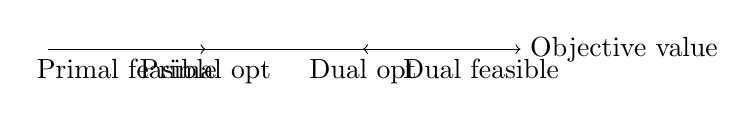
\begin{tikzpicture}
    \draw[->] (-3,0) -- (3,0) node[right] {Objective value};
    \node at (-2,0) [below] {Primal feasible};
    \node at (-1,0) [below] {Primal opt};
    \node at (1,0) [below] {Dual opt};
    \node at (2.5,0) [below] {Dual feasible};
    \draw[->] (-3,0) -- (-1,0);
    \draw[->] (3,0) -- (1,0);
\end{tikzpicture}
\end{center}
a) Weak: Let \(x\) be any feasible solution to the primal LP, and let \(y\) be any feasible solution to its dual LP. Then
\[
\sum_{j = 1}^{n}c_{j}x_{j}\leq \sum_{i = 1}^{m}b_{i}y_{i}
\]
Proof.
\[
\sum_{j = 1}^{n}c_{j}x_{j}\leq \sum_{j = 1}^{n}\left(\sum_{i = 1}^{m}a_{ij}y_{i}\right)x_{j} = \sum_{i = 1}^{m}\left(\sum_{j = 1}^{n}a_{ij}x_{j}\right)y_{i}\leq \sum_{i = 1}^{m}b_{i}y_{i}
\]
b) Strong: \(x\) and \(y\) are optimal solutions to primal and dual LPs respectively iff
\[
\sum_{j = 1}^{n}c_{j}x_{j} = \sum_{i = 1}^{m}b_{i}y_{i}
\]
Proof. \((\Longleftarrow)\) According to weak duality theorem, neither solution can be improved further, thus optimal solutions. \((\Rightarrow)\) involves using Simplex Method. Omitted. (not- required).

10. \textbf{Simplex Method}.
a) Definitions.
    i. Linear constraints form the boundary as a polyhedron, consisting of hyperplanes.
    ii. Vertex is the point at which some hyperplanes meet.
    iii. Two vertices are neighbors if they are adjacent on the polyhedron.
b) Key Idea. Start at a vertex; compare objective value with the neighbors; Move to neighbors that improves objective function, and repeat the previous step; if no improving neighbor, then stop.
c) Time Complexity. Efficient in practice, but exponential in worst case.
d) (just-to-know) Other method such as Interior Point Algorithms can reach \(O(n^4 L)\) (Ellipsoid Algorithm) or even \(O(n^{3.5}L)\) (Karmarkar's Algorithm).
e) How to perform Simplex Method?
    Step 1. Converting LP into slack form; non- basic variables is in the objective, and basic variables are the new variables in the constraints.
    Step 2. Obtaining basic solutions. Setting all non- basic variables to 0;
    Step 3. Selecting non- basic variable \(x_{e}\) with positive coefficient in \(f(x_{1},x_{2})\) , and increase the value of \(x_{e}\) without violating constraints.
    Step 4. Pivoting: exchange a non- basic variable (often \(x_{e}\) ) and a basic variable (often the corresponding variable).
    Step 5. Repeat Step 2 to Step 4 until the coefficient of non- basic variables all have negative coefficient.
(For further information, refer to CLRS books in Reference 12)

\section*{Slide 09: Amortized Analysis}

1. Amortized Analysis: a strategy to give a tighter bound evenly for a sequence of operations under worst case scenario; Basic idea: "spread out" the cost of expensive operations to all operations. If the artificial amortized costs are still cheap, then we can get a tighter bound overall.
Difference with average-case analysis: The former one is average on operations; the latter one is average over all input.
Types: Aggregate analysis; Accounting method; Potential method.
Basic Idea: for each operation, we assign an amortized cost \(\hat{C}_{i}\) to bound the actual cost, then for any sequence of \(n\) operations, we have (\(C_{i}\) is the actual cost)
\[
T(n) = \sum_{i = 1}^{n}C_{i}\leq \sum_{i = 1}^{n}\hat{C}_{i}
\]
Then all the operations have the same amortized cost \(\frac{1}{n}\sum_{i = 1}^{n}\hat{C}_{i}\).

2. \textbf{Aggregate Analysis}: sum up all the cost of operations, and then perform amortized analysis.
a) Example: Stack with multi-pop operations.
Key Observation. \(\# Pop\leq \# Push\) . Therefore, \(T(n)\leq 2\# Push\) . Amortized \(O(1)\) time for each operation.

3. \textbf{Accounting Method}: if \(\widehat{C}_{i} > C_{i}\) , the overcharge will be stored as prepaid credit; the credit will be used later for the operations with \(\widehat{C}_{i} < C_{i}\) . We need to assume that credit never goes negative.
a) Example: Stack with multi- pop operations.
Solution. Every time we push an element into the stack, we store an extra credit used in pop / multi- pop operations.
b) Example: Incrementing a binary counter.
Solution. Every time we flip a bit from 0 to 1, we store an extra credit used to flip the bit back to 0.
Observation. In every operation, we can only flip one bit from 0 to 1!

4. \textbf{Potential Function Method}: define a potential function as a bridge, i.e., we can assign a value to state rather than operation, and amortized costs are then calculated based on potential function.
Potential Function: \(\Phi (S):S\to R\) ,where \(S\) is state collection.
Amortized Cost Setting: \(\widehat{C}_{i} = C_{i} + \Phi (S_{i}) - \Phi (S_{i - 1})\)
Final Cost:
\[
\sum_{i = 1}^{n}\widehat{C}_{i} = \sum_{i = 1}^{n}\left(C_{i} + \Phi (S_{i}) - \Phi (S_{i - 1})\right) = \Phi (S_{n}) - \Phi (S_{0}) + \sum_{i = 1}^{n}C_{i}
\]
Therefore, if \(\Phi (S_{n})\geq \Phi (S_{0})\) , we can guarantee that \(\sum_{i = 1}^{n}C_{i}\leq \sum_{i = 1}^{n}\widehat{C}_{i}\)
So it is also our goal to find a potential function satisfying \(\Phi (S_{n})\geq \Phi (S_{0})\) , and \(\widehat{C}_{i}\) is a constant number.
a) Example: Stack with multi-pop operations.
Solution. Set "credit" as potential function.
Correctness. \(\Phi (S_{i})\geq 0 = \Phi (S_{0})\) for all \(i\).
Amortized Cost. push: 2; pop: 0; multi- pop: 0.
b) Example: Incrementing a binary counter.
Solution. \(\Phi (S) = \# 1\) in counter.
Correctness. \(\Phi (S_{i})\geq 0 = \Phi (S_{0})\) for all \(i\).
Amortized Cost. Increment:
\begin{align*}
\widehat{C}_{i} &= C_{i} + \Phi (S_{i}) - \Phi (S_{i - 1}) = 1 + \# \mathrm{flip}_{1\to 0} \\
\Phi (S_{i}) &= \Phi (S_{i - 1}) + 1 - \# \mathrm{flip}_{1\to 0}
\end{align*}
Therefore, \(\widehat{C}_{i} = 2\).

[Lab 07 / 1] Potential function method.
[Lab 07 / 2] Potential function method (not so convenient).

5. Example: \textbf{Dynamic Tables} - insert only.
Observation. Expansions are rare.
a) Aggregate analysis: find out the time when table expands.
\[
\sum_{i = 1}^{n}C_{i} = n + \sum_{j = 0}^{\lceil \lg n\rceil}2^{j}\leq n + 2n = 3n
\]
b) Accounting method: amortized cost \(\widehat{C}_{i} = 3\) : 1 pays for the insertion itself; 2 is stored for later table doubling, 1 for copying one of the recent half items, and 1 for copying one of the old half items.
Key Observation. The credit never goes negative.
c) Potential function. the bank account can be view as the potential function. After an expansion, \(\Phi (T) = 0\) immediately before an expansion, \(\Phi (T) = size[T]\) (Then the cost can be eliminated by the delta of \(\Phi\) ). Therefore,
\[
\Phi (T) = 2num[T] - size[T]
\]
Correctness. The table never contains less than half elements. Therefore \(\Phi (S_{i})\geq 0 = \Phi (S_{0})\) for all \(i\).
Amortized Cost. Insert but no expansion: 3; Insert with expansion: 3.

6. Example: Dynamic Tables - insert and delete.
Design. The load factor \(\alpha (T)\) never drops below \(1 / 4\) .
Potential function. Similarly,
\begin{align*}
\Phi (T) &= \frac{1}{2} size[T] - num[T] \quad (\alpha (T)< \frac{1}{2}) \\
\Phi (T) &= 2num[T] - size[T] \quad (\alpha (T)\geq \frac{1}{2})
\end{align*}
Correctness. According to the design, \(\Phi (S_i)\geq 0 = \Phi (S_0)\) for all \(i\) .
Amortized Cost. Insert, no less than \(1 / 2\) , no expansion: 3; insert, no less than \(1 / 2\) , expansion: 3; insert, less than \(1 / 2\) , and still less than \(1 / 2\) : 0; insert, less than \(1 / 2\) , then no less than \(1 / 2\) : 0. Delete, less than \(1 / 2\) , no contraction: 2; delete, less than \(1 / 2\) , contraction: 1; delete, no less than \(1 / 2\) , still no less than \(1 / 2\) , - 1; delete, no less than \(1 / 2\) , less than \(1 / 2\) , 2. (Refer to slide for detailed calculation.)

\section*{Slide 10: Graph Algorithm}

1. Definitions \& Basic Theorem.
a) Vertex, directed (undirected) edge (arcs);
b) Path, cycle;
c) Directed (undirected) graph;
d) Strongly Connected Component: every vertex is reachable from every other vertex;
e) Subgraph \(H\subset G\) : spanning/induced subgraph.
f) Handshaking Theorem:
\[
\sum_{v\in V}d(v) = 2|E|
\]

2. Notations.
a) Complete Graph: \(K_{n}\)
b) Bipartite Graph: \(K_{m,n}\)
c) Star: \(K_{1,n}\)
d) r-Partite Graph: \(K_{r(m)}\)

3. Algorithms.
a) Graph Decomposition: Depth-First Search (Topological Sort, DAG, Stack); Breadth-First Search (Cardinality Shortest Path, Queue); Minimum Spanning Tree (Prim, Kruskal, Circle-Delete);
b) Shortest Path: Single-Source Shortest Path (Dijkstra, Bellman-Ford); All-Pairs Shortest Path (Matrix, Floyd-Warshall, Johnson's);
c) Maximum Flow: Max-Flow Min-Cut Theorem; Ford-Fulkerson Algorithm; Edmond-Karp Enhancement (Augmenting Path).

4. \textbf{Minimum Spanning Tree}
a) \textbf{Prim}: maintain an optimal tree. Maintain two vertex sets \(A,B\) initially \(A\) contains one vertex and \(B\) contains others. Every time we choose the minimum-weight edge linking a vertex from \(A\) and a vertex from \(B\) , and add both vertex to \(A\) , until \(A = V\) . Therefore, the result is the MST.
Proof: by perform substitution to the "cycle", and get a MST with less weight, which contradicts the definition.
b) \textbf{Kruskal}: sort edge in an increasing order, use disjoint set to maintain min-weight acyclic edge set;
Proof: by induction on the following proposition: If \(F\) is the set of edges chosen at any stage of the algorithm, then there is some minimum spanning tree that contains \(F\) and none of the edges rejected by the algorithm.
c) \textbf{Reverse-Delete}: circle-deletion, reversed-kruskal. sort edge in a decreasing order, every time we try to delete a edge and check whether the rest of the graph is still connected (if yes, delete; if no, in MST).
Proof: similar to the proof of Kruskal algorithm; by induction on the similar proposition.
d) \textbf{Boruvka Algorithm}: maintain the cheapest edge in each components, and then add all cheapest edge into the MST. Refer to Wikipedia for details.
e) General Proof Method: cycle/cut property.
f) Efficiency Improvement: (time complexity) heap.

[Lab 07 / 3] Use cycle/cut property to prove the MST.

\section*{Slide 11: Graph Decompositions}

1. Depth-First Search in Undirected Graph.
a) Graph Explore: pre-visit \& post-visit label of each vertex.
\begin{algorithm}
\caption{EXPLORE\((G, v)\)}
\begin{algorithmic}[1]
\Input \(G = (V,E)\) is a graph; \(v \in V\)
\Output VISITED\((u) = true\) for all nodes \(u\) reachable from \(v\)
\State VISITED\((v) = true\);
\State PREVISIT\((v)\);
\For{each edge \((v, u) \in E\)}
    \If{not VISITED\((u)\)}
        \State EXPLORE\((G, u)\);
    \EndIf
\EndFor
\State POSTVISIT\((v)\);
\end{algorithmic}
\end{algorithm}

b) DFS procedure:
\begin{algorithm}
\caption{DFS\((G)\)}
\begin{algorithmic}[1]
\Input \(G = (V,E)\) is a graph
\Output VISITED\((v)\) is set to \(true\) for all nodes \(v \in V\)
\For{each \(v \in V\)}
    \State VISITED\((v) = false\);
\EndFor
\For{each \(v \in V\)}
    \If{not VISITED\((v)\)}
        \State EXPLORE\((G, v)\);
    \EndIf
\EndFor
\end{algorithmic}
\end{algorithm}

c) Time Complexity: \(O(|V| + |E|)\).
d) Connectivity in Undirected Graph: record a connected component number for each vertex, when they are visited (after pre-visit), set the number to \(cc\) , which is the current connected component number. Initial \(cc = 0\) , and every time we call explore (G, v), we increase \(cc\) by 1.
e) In both pre-visit and post-visit, we maintain a clock timestamp indicates the current time (the pre-visit/post-visit number of the vertex), then we have the following lemma.
Lemma. \(\forall u,v\in V\) \([pre(u),post(u)]\) \([pre(v),post(v)]\) are either disjoint or one is contained within the other.
Proof. If u is an ancestor of v (or v is an ancestor of u), then one is contained within the other; otherwise two intervals must be disjoint (according to the property of DFS, "return only all adjacent vertices are visited").

2. \textbf{Depth-First Search in Directed Graph}.
a) DFS yields a search tree/forests: root; parent and child; descendant and ancestor. Types of edges:
    i. Tree edges: part of the DFS forest;
    ii. Forward edges: lead from a node to a nonchild descendant in the DFS tree;
    iii. Back edges: lead to an ancestor in the DFS tree;
    iv. Cross edges: neither descendant nor ancestor; leading to a node that has already been explored.
\begin{center}
\begin{tabular}{|c|c|}
\hline
\textbf{PRE/POST ordering for \((u, v)\)} & \textbf{Edge type} \\
\hline
\([u \quad [v \quad ]v \quad ]u\) & Tree/forward \\
\([v \quad [u \quad ]u \quad ]v\) & Back \\
\([v \quad ]v \quad [u \quad ]u\) & Cross \\
\hline
\end{tabular}
\end{center}
b) Lemma. A directed graph has a cycle iff its DFS tree has a back edge.
Proof. \((\Leftarrow)\) Obviously; \((\Rightarrow)\) Focus on the first discovered vertex in the cycle, then the previous edge is a back edge.
c) Linearization / Topologically Sort. Order the vertices such that every edge goes from a small vertex to a large one.
Lemma. In a DAG, every edge leads to a vertex with a lower post number.
Proof. Use the previous lemma, since DAG is acyclic, then no back edge, thus proved.
Lemma. Every DAG has at least one source and at least one sink, where sink is a vertex with no outgoing edges, and source is a vertex with no incoming edges.
Proof. Or it will form a cycle.
Algorithm. (Topological Sort) Find a source, output it, and delete it from the graph; repeat until the graph is empty.

[Lab 08 / 3] Topological Sort + Simple DP.

d) Strongly Connected Components. Two nodes \(u\) , \(v\) in a directed graph are connected if there is a path from \(u\) to \(v\) and a path from \(v\) to \(u\) . This relation partitions \(V\) into disjoint sets that we call strongly connected components.
Lemma. Every directed graph is a DAG of its strongly connected components.
Proof. Obviously, cycles are only in the strongly connected components. So if we regard SCC as a meta- node, then the graph is acyclic, therefore DAG.
Lemma. If the explore subroutine is started at node \(u\) , then it will terminate precisely when all nodes reachable from \(u\) have been visited.
Proof. (by contradiction) Obvious.
Lemma. If \(C\) and \(C'\) are SCCs, and there is an edge from a node in \(C\) to a node in \(C'\) , then the highest post number in \(C\) is bigger than the highest post number in \(C'\) .
Proof. If we discover \(C\) first, then we will terminate visiting \(C\) after we terminate visiting \(C'\) . If we discover \(C'\) first, then the lemma is obviously correct.
Lemma. The node that receives the highest post number in DFS must lies in a source SCC.
Proof. Obvious according to the previous lemma.
Note. The smallest post number in DFS may not lie in a sink SCC! Possible counterexamples:
\begin{center}
    % Placeholder for the image in the PDF
    \framebox{\parbox{0.6\textwidth}{\centering \textit{[Diagram of SCC counterexample]}}}
\end{center}

[Lab 08 / 2] Similar definitions: biconnected components, articulation points and bridges.

e) \textbf{Kosaraju Algorithm}. Consider the reverse graph \(G^{R}\) , the same as \(G\) but with all edges reversed, then it has exactly the same SCCs as \(G\) . Therefore, its sink SCC is the source SCC in \(G\) . Perform DFS on \(G^{R}\) and get post number, and run DFS on \(G\) and process the vertices in decreasing order of their previous post number in the last step.
Time Complexity: \(O(|V| + |E|)\) . Since DFS has a linear time complexity.

[Lab 09 / 2] The implementation of the Kosaraju Algorithm.

3. \textbf{Breadth-First Search}: use a queue to store the current vertices.
\begin{algorithm}
\caption{BFS\((G, s)\)}
\begin{algorithmic}[1]
\Input Graph \(G = (V, E)\), directed or undirected; vertex \(s \in V\)
\Output DIST\((u)\) is set to the distance from \(s\) to all reachable \(u\)
\For{each \(u \in V\)}
    \State DIST\((u) = \infty\);
\EndFor
\State DIST\((s) = 0\);
\State \(Q = [s]\) (queue containing just \(s\));
\While{\(Q\) is not empty}
    \State \(u = \text{EJECT}(Q)\);
    \For{each edge \((u, v) \in E\)}
        \If{DIST\((v) = \infty\)}
            \State INJECT\((Q, v)\);
            \State DIST\((v) = \text{DIST}(u) + 1\);
        \EndIf
    \EndFor
\EndWhile
\end{algorithmic}
\end{algorithm}

a) Lemma. For each \(d = 0,1,2,\dots\) there is a moment at which
(1) all nodes at distance \(\leq d\) from \(s\) have their distances correctly set;
(2) all other nodes have their distance set to \(\infty\) ;
(3) the queue contains exactly the nodes at distance \(d\) .
Proof. The moment is exactly after the nodes at distance \(\leq d - 1\) are visited.
b) Lemma. BFS has a running time of \(O(|V| + |E|)\) .
Proof. the dist array acts like the visit array in DFS, therefore every vertex can only be visited once.

[Lab 08 / 1] Similar to DFS tree/forest, BFS tree/forest has some properties.

\section*{Slide 12: Shortest Path}

1. Definition \& Properties.
a) The weight of a path: the summation of edge weights.
b) The shortest path from u to v: a path of minimum weight from u to v. The shortest path weight from u to v is defined as \(d(u,v) = \min \{w(P) | P\) is a path from u to v}; specially, if no path exists, then \(d(u,v) = +\infty\) .
c) Optimal Substructure: A subpath of a shortest path is a shortest path.
Proof. (by contradiction) Or we can construct a shorter path.
d) Triangle Inequality: \(\forall v_1,v_2,v_3\in V,d(v_1,v_2)\leq d(v_1,v_3) + d(v_3,v_2)\) .
Proof. (by contradiction) Obvious.
e) If a graph G contains a negative- weight cycle, then some shortest path may not exist.

2. \textbf{Single Source Shortest Path (SSSP)}: from a given source vertex s, find the shortest- path weights \(d(s,v)\) for all \(v\in V\) .
a) If all edge weights are non- negative, all shortest- path weights must exist; otherwise the shortest- path weights may not exist because of the negative cycle. (non- negative weight: Dijkstra's Algorithm; negative weight: Bellman- Ford Algorithm).
b) \textbf{Dijkstra Algorithm}. (Greedy) maintain a set \(S\) of vertices whose shortest- path distances from \(s\) are known; at each step add to \(S\) the vertex \(v\in V\backslash S\) whose distance estimate from \(s\) is minimal; update the distance estimates of vertices adjacent to \(v\) . Negative weights is NOT allowed. Re- weighting of negative weights fails.

\begin{algorithm}
\caption{Dijkstra's Algorithm}
\begin{algorithmic}[1]
\For{each \(u \in V\)}
    \State INSERT \((Q,u)\)
\EndFor
\While{\(Q \neq \emptyset\)}
    \State \(u \leftarrow \text{EXTRACT-MIN}(Q)\)
    \State \(S \leftarrow S \cup \{u\}\)
    \For{each \(v \in Ad[u]\)}
        \If{\(d[v] > d[u] + w(u,v)\)}
            \State \(d[v] \leftarrow d[u] + w(u,v)\) \Comment{Relaxation Step}
            \State DECREASE-KEY \((Q,v)\)
        \EndIf
    \EndFor
\EndWhile
\end{algorithmic}
\end{algorithm}

Lemma. Initializing \(d[s]\gets 0\) and \(d[v]\gets +\infty\) for all \(v\in V\backslash \{s\}\) establishes \(d[v]\geq d(s,v)\) for all \(v\in V\) and this invariant is maintained over any sequence of relaxation steps.
Proof. (by contradiction) suppose not, then \(d[v]< d(s,v)\) , suppose \(v\) is updated by \(u\) , then \(d[v] = d[u] + w(u,v)\) but, \(d[v]< d(s,v)\leq d(s,u) + w(u,v)\leq d[u] + w(u,v)\) which derives a contradiction.
Theorem. Dijkstra algorithm terminates with \(d[v] = d(s,v)\) for all \(v\in V\) .
Proof. It suffices to show that \(d[v] = d(s,v)\) for every \(v\in V\) when \(v\) is added to \(S\) . Suppose \(u\) is the first vertex added to \(S\) for which \(d[u]\neq d(s,u)\) . Let \(y\) be the first vertex in \(V\backslash S\) along a shortest path from \(s\) to \(u\) , and let \(x\) be its predecessor. Therefore, we have \(d[x] = d(s,x)\) and \(d[y] = d(s,x) + w(x,y) = d[x] + w(x,y)\) since the sub- path of the shortest path is a shortest path. Therefore, \(d[y]\) was set to \(d(s,y)\) when \((x,y)\) was relaxed after \(x\) was added to \(S\) . Hence, \(d[y] = d(s,y)\leq d(s,u)\leq d[u]\) . However, we choose \(u\) instead of \(y\) in the algorithm, which means \(d[u]\leq d[y]\) . Therefore, \(d[y] = d(s,y) = d(s,u) = d[u]\) , which contradicts the premise.

\begin{center}
    % Placeholder for the image in the PDF
    \framebox{\parbox{0.5\textwidth}{\centering \textit{[Diagram for Dijkstra proof]}}}
\end{center}

Complexity Analysis. Totally \(O(|E|)\) DECREASE- KEY and \(O(|V|)\) EXTRACT- MIN. If we use binary heap, we can reach the time complexity of \(O((|V| + |E|)\log |V|)\) , but if we use Fibonacci heap, it can be optimized to \(O(|V|\log |V| + |E|)\) (just- to- know).
c) Dijkstra Algorithm in unweighted graph. Use FIFO queue instead of priority queue (BFS), linear time complexity.
d) \textbf{Bellman-Ford Algorithm}. Dynamic Programming Approach, negative weights is allowed.
Let \(f(i,v)\) denote the length of the shortest \(s\) - v path \(P\) using at most \(i\) edges.
\[
f(i,v) = \min \left\{f(i - 1,v),\min_{(u,v)\in E}\{f(i - 1,u) + w(u,v)\}\right\}
\]
Initially, \(f(\cdot ,s) = 0,f(0,v) = +\infty\) \((v\neq s)\) .
Improvements. maintain only one \(f(v)\) as the shortest \(s\) - v path found so far, less space complexity; no need to check edges of the form \((u,v)\) unless \(f(u)\) changed.
\begin{algorithm}
\caption{Bellman-Ford Algorithm}
\begin{algorithmic}[1]
\For{each node \(u \in V\)}
    \State \(M[u] \leftarrow \infty\);
    \State \(predecessor[u] \leftarrow \emptyset\);
\EndFor
\State \(M[s] \leftarrow 0\);
\For{\(i = 1\) to \(n - 1\)}
    \For{each node \(u \in V\)}
        \If{\(M[u]\) has been updated in previous iteration}
            \For{each edge \((u,v) \in E\)}
                \If{\(M[v] > M[u] + w(u,v)\)}
                    \State \(M[v] \leftarrow M[u] + w(u,v)\);
                    \State \(predecessor[v] \leftarrow u\);
                \EndIf
            \EndFor
        \EndIf
    \EndFor
    \If{No \(M[v]\) changed in this iteration, stop.}
\EndFor
\end{algorithmic}
\end{algorithm}
Theorem. Throughout the algorithm, \(f(v)\) is length of some \(s\) - v path, and after \(i\) rounds of updates, the value of \(f(v)\) is no larger than the length of shortest \(s\) - v path using \(\leq i\) edges.
Proof. Obviously according to dynamic programming and the algorithm.
Time Complexity. \(O(mn)\) time worst case, but substantially faster in practice; \(O(m + n)\) spaces.
Lemma. If \(f(n,v) = f(n - 1,v)\) for all \(v\) , then no negative cycle in the graph;
Proof. Bellman- Ford Algorithm.
Lemma. If \(f(n,v)< f(n - 1,v)\) for some \(v\) , then shortest path from \(s\) to \(v\) contains a negative- weighted cycle \(W\) .
Proof. Obvious according to the pigeonhole principle and the premise.
Theorem. Negative cycle detection algorithm in \(O(mn)\) time using Bellman- Ford Algorithm. Add new node \(s\) and connect it to all nodes with 0- cost edge, and check if \(f(n,u) = f(n - 1,u)\) for all \(u\) . If no, then extract cycle from shortest path from \(s\) to \(u\) .

3. \textbf{All-Pair Shortest Path}: find the shortest- path weights \(d(u,v)\) for all \(u,v\in V\) .
a) Run Bellman-Ford once from each vertex: \(O(n^{2}m)\) , in dense graph, \(O(n^{4})\) .
b) Matrix Multiplication: consider \(n\times n\) adjacency matrix \(A = (a_{ij})\) of the digraph, and define \(d_{ij}^{(m)}\) as the weight of a shortest path from \(i\) to \(j\) that uses at most \(m\) edges. Therefore,
\[
d_{ij}^{(m)} = \min_k\left\{d_{ik}^{(m - 1)} + a_{kj}\right\}
\]
No negative- weight cycles implies: \(d(i,j) = d_{ij}^{(n - 1)} = d_{ij}^{(n)} = \dots\) .
Notice the formula is like matrix multiplication, except change sum to min, and change multiplying to adding. Since \((\min, +)\) is also associative, then it is a closed semiring. Therefore, we just need to "multiply" it \(n\) times. Using Quick Power method, we can optimize it to \(O(n^{3}\log n)\) .
c) \textbf{Floyd-Warshall Algorithm}: Define \(c_{ij}^{(k)}\) as the weight of a shortest path from \(i\) to \(j\) with intermediate vertices belonging to the set \(\{1,2,\ldots ,k\}\) . Thus, \(d(i,j) = c_{ij}^{(n)}\) and \(c_{ij}^{(0)} = a_{ij}\) .
\[
c_{ij}^{(k)} = \min_k\left\{c_{ij}^{(k - 1)},c_{ik}^{(k - 1)} + c_{kj}^{(k - 1)}\right\}
\]
Note. Enumerate \(k\) first!
Time Complexity. \(O(n^3)\) , simple and efficient.
[Lab 09 / 1] The shortest path matrix updation.
d) Transitive Closure of a Directed Graph. Compute if there exists a path (1 - yes, 0 - no) for each pair of vertices. Using Floyd-Warshall Algorithm, but replace \((\min, +)\) with \((\lor, \land)\) .
e) \textbf{Johnson's Algorithm}. Bellman-Ford for graph re-weighting and Dijkstra for shortest path.
Graph Re- weighting Theorem. Given a label \(h(\nu)\) for each \(\nu \in V\) , re- weight each edge \((u,\nu)\in E\) by
\[
\bar{\omega} (u,\nu) = w(u,\nu) + h(u) - h(\nu)
\]
Then, all paths between the same two vertices \(x\) and \(y\) are reweighted by the same amount (add \(h(x) - h(y))\) .
Proof. Obvious by summation.
Algorithm.
1) Find a vertex labeling \(h\) such that \(\bar{\omega} (u,\nu)\geq 0\) for all \((u,\nu)\in E\) by using Bellman-Ford to solve the constraints
\[
h(\nu) - h(u)\leq w(u,\nu)
\]
or determine that a negative- weight cycle exists. \(h(\cdot)\) is actually the original \(d(\cdot)\) .
Time Complexity. \(O(mn)\) .
2) Run Dijkstra algorithm from each vertex using \(\bar{\omega}\) .
Time Complexity: \(O(mn + n^2\log n)\) using Fibonacci heap.
3) Re-weight each shortest-path length \(\bar{\omega} (P)\) and produce the actual shortest-path length \(w(P)\) .
Time Complexity: \(O(n^2)\) .
Full Time Complexity. \(O(mn + n^2\log n)\) (using Fibonacci heap in Dijkstra).

\section*{Slide 13: Network Flow}

1. \textbf{Flow Network}. A flow network is a tuple \(G = (V,E,s,t,c)\) .
a) Directed Graph \(G = (V,E)\) with source \(s\in V\) and sink \(t\in V\) .
b) Assume all nodes are reachable from \(s\) and no parallel edges.
c) Capacity \(c(e) > 0\) for each edge \(e\in E\) .

2. Definitions.
a) \textbf{Cuts}. An \(s\) -t cut is a partition \((A,B)\) of \(V\) with \(s\in A\) and \(t\in B\) .
b) \textbf{Capacity}. The capacity of a cut \((A,B)\) is \(cap(A,B) = \sum_{e \text{ out of } A} c(e)\) . (Note: out of).
c) \textbf{Minimum \(s\) -t Cut}. Find an \(s\) -t cut of minimum capacity.
d) \textbf{Flow}. An \(s\) -t flow \(f\) is a function that satisfies:
    i. Capacity: for each \(e\in E\) \(0\leq f(e)\leq c(e)\) .
    ii. Conservation: for each \(\nu = V\backslash \{s,t\} \colon \sum_{e \text{ in to } v} f(e) = \sum_{e \text{ out of } v} f(e)\) .
e) \textbf{Value}: the value of a flow \(f\) is \(v(f) = \sum_{e \text{ out of } s} f(e) - \sum_{e \text{ in to } s} f(e)\) .
f) \textbf{Max flow problem}. Find an \(s\) -t flow of maximum value.

3. Properties.
a) \textbf{Flow Value Lemma}. Let \(f\) be any flow, and let \((A,B)\) be any \(s\) -t cut. Then, the value of \(f\) equals to the net flow across the cut \((A,B)\) , that is,
\[
v(f) = \sum_{e\mathrm{out\ of}A}f(e) - \sum_{e\mathrm{in\ to}A}f(e)
\]
Proof. By flow conservation and the definition of value.
b) \textbf{Weak Duality}. Let \(f\) be any flow. Then for any \(s\) -t cut \((A,B)\) we have
\[
v(f)\leq cap(A,B)
\]
c) Corollary. Let \(f\) be any flow, and let \((A,B)\) be any cut. If \(\nu (f) = cap(A,B)\) , then \(f\) is a max flow and \((A,B)\) is a min cut.
Proof. For any flow \(f^{\prime}\) , \(\operatorname {val}(f^{\prime})\leq \operatorname {cap}(A,B) = \operatorname {val}(f)\) , which shows that \(f\) is a max flow. For any cut \((A^{\prime},B^{\prime})\) \(\operatorname {cap}(A^{\prime},B^{\prime})\geq \operatorname {val}(f) = \operatorname {cap}(A,B)\) , which shows that \((A,B)\) is a min cut.

4. \textbf{Max-Flow Algorithm}. (Also min-cut).
a) Residual edge. For all \(e = (u,v)\in E\) , we need "undo" the flow, so we add edge \(e^{R} = (v,u)\) and residual capacity \(c_{f}(e) = c(e) - f(e)\) if \(e\in E\) . \(c_{f}(e) = f(e)\) if \(e^{R}\in E\) .
b) Residual network. \(G_{f} = (V,E_{f},s,t,c_{f})\) . Residual edges with positive residual capacity, and \(E_{f}\) contains residual edges, that is, \(E_{f} = \{e\mid f(e)< c(e)\} \cup \{e^{R}\mid f(e) > 0\}\) .
Key Property. \(f^{\prime}\) is a flow in \(G_{f}\) iff \(f\) is a flow in \(G\) .
c) Augmenting path. A simple \(s\stackrel {\leftrightarrow}{\longrightarrow}t\) path in the residual network \(G_{f}\) .
Bottleneck capacity. The bottleneck capacity of an augmenting path \(P\) is the minimum residual capacity of any edge in \(P\) .
Key Property. Let \(f\) be a flow and let \(P\) be an augmenting path in \(G_{f}\) . Then after calling \(f^{\prime}\leftarrow \operatorname {Aug}(f,c,P)\) , the resulting \(f^{\prime}\) is a flow and \(\operatorname {val}(f^{\prime}) = \operatorname {val}(f) + \operatorname {bottleneck}(G_{f},P)\) .
Augmenting subroutine.
\begin{algorithm}
\caption{AUGMENT\((f, c, P)\)}
\begin{algorithmic}[1]
\State \(\delta \leftarrow\) bottleneck capacity of augmenting path \(P\);
\For{each \(e \in P\)}
    \If{\(e \in E\)}
        \State \(f(e) \leftarrow f(e) + \delta\); \Comment{forward edge}
    \Else
        \State \(f(e^{R}) \leftarrow f(e^{R}) - \delta\); \Comment{reverse edge}
    \EndIf
\EndFor
\State \textbf{return} \(f\);
\end{algorithmic}
\end{algorithm}
d) \textbf{Ford-Fulkerson Algorithm}. Start with \(f(e) = 0\) for each \(e\in E\) . Then find a \(s\stackrel {\leftrightarrow}{\longrightarrow}t\) path \(P\in G_{f}\) , augment flow along \(P\) . Repeat until you get stuck.
\begin{algorithm}
\caption{Ford-Fulkerson Algorithm}
\begin{algorithmic}[1]
\Input \(G = (V,E), c, s, t\)
\For{each \(e \in E\)}
    \State \(f(e) \leftarrow 0\);
\EndFor
\State \(G_{f} \leftarrow\) residual graph;
\While{there exists augmenting path \(P\)}
    \State \(f \leftarrow \text{AUGMENT}(f, c, P)\);
    \State update \(G_{f}\);
\EndWhile
\State \textbf{return} \(f\);
\end{algorithmic}
\end{algorithm}
\textbf{Augmenting Path Theorem}. Flow \(f\) is a max flow iff there are no augmenting paths.
\textbf{Max- flow Min- cut Theorem}. The value of the max flow is equal to the value of the min cut.
Proof (of both). We show that the following statement is equivalent.
(1) There exists a cut \((A,B)\) such that \(\nu (f) = cap(A,B)\) .
(2) Flow \(f\) is a max flow;
(3) There is no augmenting path relative to \(f\) .
\((1)\Longrightarrow (2)\) : The corollary of the weak duality lemma;
\((2)\Longrightarrow (3)\) : Contrapositive. If there exists augmenting path, we can improve \(f\) and \(f\) is not a max flow.
\((3)\Longrightarrow (1)\) : Let \(f\) be a flow with no augmenting paths. Let \(A\) be set of vertices reachable from \(s\) in residual graph. By definition of \(A\) , \(s\in A\) . By definition of \(f\) , \(t\notin A\) .
\[
\nu (f) = \sum_{e\mathrm{out\ of}A}f(e) - \sum_{e\mathrm{in\ to}A}f(e) = \sum_{e\mathrm{out\ of}A}c(e) - \sum_{e\mathrm{in\ to}A}0 = cap(A,B)
\]
edge \(e = (v,w)\) with \(v\in B,w\in A\) must have \(f(e) = 0\) , otherwise \(e^{\prime} = (w,v)\) has capacity, and \(v\in A\) .
edge \((v,w)\) with \(v\in A,w\in B\) must have \(f(e) = c(e)\) , otherwise \(w\in A\) because there is capacity left.
Assumption. All capacities are integers between 1 and \(C\) .
Invariant. Every flow value \(f(e)\) and every residual capacity \(c_{f}(e)\) remains an integer throughout the algorithm.
Proof. by induction on the number of augmenting paths.
Theorem. The algorithm terminates at most \(\text{val}(f^*) \leq nC\) augmenting paths, where \(f^*\) is the max flow.
Proof. Each augmentation increases the value by at least 1.
Time Complexity. Ford- Fulkerson algorithms runs in \(O(nmC)\) time, because we can use BFS or DFS to find an augmenting path in \(O(m)\) time, and there are at most \(nC\) augmenting paths.
\textbf{Integrality Theorem}. There exists an integral max flow \(f\) .
Proof. Since the algorithm terminates, theorem follows from integrality invariant (and augmenting path theorem).
Note. Ford- Fulkerson algorithm is not a polynomial algorithm, since the input size is \(n,m,\log C\) .
Note. If the flow is real number instead of integer, then the algorithm may not terminate and the result may not converge to the max flow.
e) \textbf{Scaling Max-Flow Algorithm}: an improvement of FF algorithm.
Choose sufficiently large bottleneck capacity. Maintain a scaling factor \(\Delta\) , every time only find augmenting path with capacity at least \(\Delta\) (these edges construct \(G_{f}(\Delta)\) ).
\begin{algorithm}
\caption{Scaling Max-Flow Algorithm}
\begin{algorithmic}[1]
\For{each \(e \in E\)}
    \State \(f(e) \leftarrow 0\);
\EndFor
\State \(G_{f} \leftarrow\) residual graph;
\State \(\Delta \leftarrow\) smallest power of 2 greater than or equal to \(C\);
\While{\(\Delta \geq 1\)}
    \State \(G_{f}(\Delta) \leftarrow \Delta\)-residual graph;
    \While{there exists augmenting path \(P\) in \(G_{f}(\Delta)\)}
        \State \(f \leftarrow \text{ARGUMENT}(f, c, P)\);
        \State update \(G_{f}(\Delta)\);
    \EndWhile
    \State \(\Delta \leftarrow \Delta / 2\);
\EndWhile
\State \textbf{return} \(f\);
\end{algorithmic}
\end{algorithm}
Assumption. All edge capacities are integers between 1 and \(C\) .
Invariant. The scaling parameter \(\Delta\) is a power of 2.
Proof. Obvious.
Integrality Invariant. Throughout the algorithm, all flow and residual capacity values are integral.
Proof. Same as the previous proof process.
Correctness. If the algorithm terminates, then \(f\) is a max flow.
Proof. In the end, \(\Delta = 1\) , \(G_{f}(\Delta) = G_{f}\) . The algorithm stop when there is no augmenting paths, so \(f\) is a max flow.
Lemma. The outer loop repeats \((1 + \lceil \log_{2}C\rceil)\) times.
Proof. Obvious.
Lemma. Let \(f\) be the flow at the end of a \(\Delta\) - scaling phase; the value of the maximum flow is at most \(v(f) + m\Delta\) .
Proof. We show that at the end of a \(\Delta\) - phase, there exists a cut \((A,B)\) such that \(cap(A,B) \leq v(f) + m\Delta\) . Choose A to be the set of nodes reachable from \(s\) in \(G_{f}(\Delta)\) . Therefore \(s \in A\) and \(t \notin A\) .
\[
v(f) = \sum_{e\mathrm{out\ of}A}f(e) - \sum_{e\mathrm{in\ to}A}f(e)\geq \sum_{e\mathrm{out\ of}A}(c(e) - \Delta) - \sum_{e\mathrm{in\ to}A}\Delta \geq cap(A,B) - m\Delta
\]
edge \(e = (v,w)\) with \(v\in B,w\in A\) must have \(f(e)< \Delta\) , otherwise \(e^{\prime} = (w,v)\) has capacity \(\geq \Delta\) , and \(v\in A\) .
edge \((v,w)\) with \(v\in A,w\in B\) must have \(c(e) - f(e)< \Delta\) , otherwise \(w\in A\) because there is capacity left.
Lemma. There are at most \(2m\) augmentations per scaling phase.
Proof. According to the previous lemma, let \(f\) be the flow at the end of the previous scaling phase, then
\[
v(f^{\prime})\leq v(f) + m(2\Delta)
\]
Each augmentation in a \(\Delta\) - phase increases \(v(f)\) by at least \(\Delta\) .
Time Complexity. The scaling max- flow algorithm finds a max flow in \(O(m\log C)\) augmentations. It can be implemented to run in \(O(m^{2}\log C)\) time, now it is polynomial!

[Lab 09 / 3] Min- Cost- Max- Flow Problem: Each time choose a least cost augmenting paths. How to prove? No negative cycles during the process (the residual graph also has no negative cycles). Then if not optimal, say another flow \(g\) . Then we can modify \(f\) to \(g\) and there are only positive cost changes in \(f\) 's residual graph. Therefore \(g\) improves \(f\) . We can also add a new source and sink and force a flow of value \(k\) to go through, and use the Min-Cost-Max-Flow algorithm.

\section*{Slide 15: Turing Machine}

1. Effective procedure: a mechanical rule, or automatic method, or program for performing some mathematical operations. It can be viewed as a black box taking inputs and producing outputs.
Counterexample. \(g(n) =\) [there is a run of exactly \(n\) consecutive \(7^{\prime}s\) in the decimal expansion of \(\pi\) ] . The procedure may never terminate, or we do not know when does it terminate. Therefore, not "effective procedure".
Note. The answer is unknown \(\neq\) the answer is negative.
Another example. \(g(n)\) only defined when there is a run of exactly \(n\) consecutive \(7^{\prime}s\) in the decimal expansion of \(\pi\) then it is an effective procedure!
Other examples: Theorem Proving is general but not effective. But proof verification is effective!

2. Algorithm. An algorithm is a procedure that consists of a finite set of instructions which, given an input from some set of possible inputs, enables us to obtain an output through a systematic execution of the instructions that terminates in a finite number of steps.

3. Computable Function. When an algorithm or effective procedure is used to calculate the value of a numerical function then the function is effectively calculable (or algorithmically computable, effectively computable, computable).

4. Famous Computation Models: Church (1936): \(\lambda\) -Calculus; Godel- Kleene (1936): Recursive Functions; Turing (1936): Turing Machines; Post (1943) Post Systems; Shepherdson- Sturgis (1963): Unlimited Register Machine (URM can accept many states). (This part was introduced before in Slide 02. )

5. Church- Turing Thesis. Each of the above proposals for a characterization of the notion of effective computability gives rise to the same class of functions. (This part was also introduced before in Slide 02. )

6. \textbf{One-Tape Turing Machine}.
a) A Turing machine has five components.
    i. A finite set \(\{s_1,s_2,\dots,s_n\} \cup \{\square ,\triangleright \} \cup \{0,1\}\) of symbols;
    ii. A tape consists of an infinite number of cells, each cell may store a symbol;
    iii. A reading head that scans and writes on the cells; the reading head may write a symbol, move left or move right.
    iv. A finite set \(\{q_s,q_1,q_2,\dots,q_m,q_H\}\) of states.
    v. A finite set of instructions (specification).
b) An instruction is of the form: \((q_{l},s_{j})\rightarrow (q_{l},s_{k},L \text{ or } R \text{ or } S)\) which means when reads \(s_j\) with state \(q_{l}\) , the machine will turn to state \(q_{l}\) , replace \(s_j\) with \(s_k\) , and turn one cell to the left/right/stay at the current position.
c) State Transition Diagram. Draw every instruction (transitions) in a diagram.

[Lab 10 / 1] One-tape TM design.

7. \textbf{Multi-Tape Turing Machine}. A multi-tape TM is described by a tuple \((\Gamma ,Q,\delta)\) containing
a) A finite set \(\Gamma\) called alphabet, of symbols. It contains a blank symbol \(\square\) , a start symbol \(\triangleright\) and the digit 0 and 1;
b) A finite set \(Q\) of states. It contains a start state \(q_{start}\) and a halting state \(q_{halt}\) .
c) A transition function \(\delta :Q\times \Gamma^{k}\rightarrow Q\times \Gamma^{k - 1}\times \{L,S,R\}^{k}\) (the first tape is usually input tape, not for writing).

8. TM Variations.
a) Language system. Let \(\Sigma = \{a_1,a_2,\dots,a_k\}\) be the set of symbols, called alphabet. A string (word) from \(\Sigma\) is a sequence \(a_{i_1}a_{i_2}\dots a_{i_n}\) of symbols from \(\Sigma\) . \(\Sigma^{*}\) is the set of all words/strings from \(\Sigma\) (Kleene Star). For example, \(\Sigma = \{a,b\} ,\Sigma^{*} = \{a,b\}^{*} = \{\Lambda ,a,b,aa,ab,ba,bb,\dots \}\) . \(\Lambda\) is the empty string, that has no symbols (\(\epsilon\)).
\textbf{Fact}. If \(f:\{0,1\}^{*} \to \{0,1\}^{*}\) is computable in time \(T(n)\) by a TM \(M\) using the alphabet set \(\Gamma\) , then it is computable in time \(4\log|\Gamma|T(n)\) by a TM \(\tilde{M}\) using the alphabet \(\{0,1,\square,\triangleright\}\).
\textbf{Idea}. To represent a symbol with \(\log|\Gamma|\) blocks.
\textbf{Simulation}. To simulate on step of the language system TM \(M\), our one-tape TM \(\tilde{M}\) will:
    1. use \(\log|\Gamma|\) steps to read from each tape the \(\log|\Gamma|\) bits encoding a symbol of \(\Gamma\);
    2. use its state register to store the symbols read;
    3. use \(M\)'s transition function to compute the symbols \(M\) writes and \(M\)'s new state given this information;
    4. store this information in its state register;
    5. use \(\log|\Gamma|\) steps to write the encodings of these symbols on its tapes.

[Lab 10 / 2] Language system transform to simple TM.

b) \textbf{Multi-Tape TM}.
\textbf{Fact}. If \(f:\{0,1\}^{*} \to \{0,1\}^{*}\) is computable in time \(T(n)\) by a TM \(M\) using \(k\) tapes, then it is computable in time \(5k T(n)^2\) by a single-tape TM \(\tilde{M}\).
\textbf{Idea}. To interleave \(k\) tapes into one. Suppose the first tape is \(a_1 a_2 ...\), the second tape is \(b_1 b_2 ...\), the third tape is \(c_1 c_2 ...\), then the final tape is \(a_1 \hat{b_1} c_1 a_2 \hat{b_2} c_2 ...\). Also, every symbol \(a, \hat{a}\) in \(M\) is turned into two symbols \(a, \hat{a}\) in \(\tilde{M}\), with \(\hat{a}\) used to indicate head position.
\textbf{Simulation}. To simulate on step of the language system TM \(M\), our one-tape TM \(\tilde{M}\) will:
    1. The machine \(\tilde{M}\) places \(\triangleright\) after the input string and then starts copying the input bits to the imaginary input tape. During this process whenever an input symbol is copied, it is overwritten by \(\triangleright\);
    2. \(\tilde{M}\) marks the \((n + 2)\)-th cell, ..., the \((n + k)\)-th cell to indicate the initial head positions.
    3. \(\tilde{M}\) sweeps \(kT(n)\) cells from the \((n + 1)\)-th cell to right, recording in the register the \(k\) symbols marked with the hat \(\hat{}\) ;
    4. \(\tilde{M}\) sweeps \(kT(n)\) cells from right to left to update using the transitions of \(M\). Whenever it comes across a symbol with hat, it moves right \(k\) cells, and then moves left to update.

c) \textbf{Unidirectional Tape TM}.
\textbf{Fact}. If \(f:\{0,1\}^{*} \to \{0,1\}^{*}\) is computable in time \(T(n)\) by a bidirectional TM \(M\), then it is computable in time \(4T(n)\) by a TM \(\tilde{M}\) with unidirectional tape.
\textbf{Idea}. \(\tilde{M}\) makes use of the alphabet \(\Gamma \times \Gamma\). Every state \(q\) of \(M\) is turned into \(\overline{q}\) and \(q\).
\textbf{Simulation}. To unidirectional tape TM will change the original transitions to:
Let \(H\) range over \(\{L,S,R\}\) and let \(-H\) defined by \(R (H = L); L (H = R); S (H = S)\).
Add. \((\overline{q}, (s,\triangleright)) \to (q, (\triangleright,\triangleright), R)\), \((q, (\triangleright,\triangleright)) \to (\overline{q}, (\triangleright,\triangleright), R)\);
Modify. \((\overline{q}, (a,b)) \to (\overline{q}^{\prime}, (a^{\prime},b^{\prime}), H)\) for all \((q,a) \to (q^{\prime}, a^{\prime}, H)\);
\((q,(a,b)) \to (q^{\prime}, (a,b^{\prime}), -H)\) for all \((q,b) \to (q^{\prime}, b^{\prime}, H)\).
Note. here we ignore the "underline" because word cannot print it.

9. \textbf{TM- Computable Function}.
Let \(M\) be a TM and \(a_1, a_2, ..., a_n, b \in \mathbb{N}\). When computation \(M(a_1,a_2,...,a_n)\) converges to \(b\) if \(M(a_1,a_2,...,a_n) \downarrow (1 \text{ means halting})\) and \(r_1 = b\) in the final configuration. We write \(M(a_1,a_2,...,a_n) \downarrow b\).
\textbf{TM-computes}. M TM-computes \(f\) if, for all \(a_1, a_2, ..., a_n, b \in \mathbb{N}\),
\[
M(a_1,a_2,...,a_n) \downarrow b \quad iff \quad f(a_1,a_2,...,a_n) = b
\]
\textbf{TM-computable}: function \(f\) is TM-computable if there is a Turing Machine that TM-computes \(f\).
\textbf{Note}. We abbreviate "TM-computable" to "computable".

10. \textbf{Function Defined by Program}. Given any program \(P\) and \(n\geq 1\) , by thinking of the effect of \(P\) on initial configurations of the form \(a_{1},a_{2},\ldots ,a_{n},0,0,\ldots\) there is a unique \(n\) -ary function that \(P\) computes, denoted by \(f_{P}^{(n)}\) .
\begin{align*}
f_{P}^{(n)} &= b \quad (P(a_{1},a_{2},\dots ,a_{n})\downarrow b) \\
f_{P}^{(n)} &= \text{undefined} \quad (P(a_{1},a_{2},\dots ,a_{n})\uparrow)
\end{align*}

11. \textbf{Decidable}: suppose a predicate \(P(x_{1},x_{2},\dots,x_{n})\) is an \(n\) -ary predicate of natural numbers. Then define the characteristic function \(c_{P}(x)\) as follows.
\[
c_{P}(x) = [P(x)\mathrm{holds}]
\]
The predicate \(P(x)\) is decidable iff \(c_{P}(x)\) is computable; otherwise it is undecidable.

12. Computability on other Domains. Suppose \(D\) is an object domain. A coding of \(D\) is an explicit and effective injection \(\alpha :D\to \mathbb{N}\) . We say that an object \(d\in D\) is coded by natural number \(\alpha (d)\) . A function \(f:D\to D\) extends to a numeric function \(f^{*}:\mathbb{N}\to \mathbb{N}\) . We say that \(f\) is computable if \(f^{*}\) is computable.
\[
f^{*} = \alpha \circ f\circ \alpha^{-1}
\]

\section*{Slide 16: NP Reduction}

1. \textbf{Decision Problem}: \(X\) is a set of strings. Instance is string \(s\) . Algorithm \(A\) solves problem \(X\) : \(A(s) = yes\) iff \(s\in X\) .

2. \textbf{Polynomial time}. Algorithm A runs in poly-time if for every string \(s\) \(A(s)\) terminates in at most \(p(|s|)\) "steps", where \(p(\cdot)\) is some polynomial and \(|s|\) is the length of \(s\) (input size).

3. \textbf{Search Problem}. \(X\) is a set of strings. Instance is string \(s\) . Feasible solution is \(s_{x}\) . Algorithm \(A\) searches the optimal solution for problem \(X\) : \(A(s) = \min \{|s_{x}|\}\) or \(\max \{|s_{x}|\}\) , \(s\in X\) .
Example. (introducing new argument \(k\) to make it a decision problem)
(Shortest- Path Problem) Does there exist a shortest path of weight no more than \(k?\)

4. \textbf{P}. Decision problems for which there is a poly-time algorithm.
Deterministic Turing Machine (DTM): is a TM \(M\) whose transaction function set has at most one instruction for each combination of symbol and state.
Another Definition of P: Decision problems that can be solved by DTM polynomially.

5. \textbf{Certifier}. Algorithm \(C(s,t)\) is a certifier for problem \(X\) if for every string \(s\) , \(s\in X\) iff there exists a string such \(t\) that \(C(s,t) = yes\) (informally, the checking program.)
Certificate. The string \(t\) used in the certifier as a checking parameter.
[Lab 11 / 1] Certificate \& Certifier.

6. \textbf{NP}. Decision problems for which there exists a poly-time certifier \((C(s,t)\) is a poly-time algorithm and \(|t|< p(|s|)\) for some polynomial \(p(\cdot)\) . (Explanation: NP stands for non-deterministic polynomial-time.)
Non-Deterministic Turing Machine (NTM): is a TM \(M\) which may have a set of specifications that prescribes more than one action for a given state.
Another Definition of NP. Decision problems that can be solved by NTM polynomially, or certificates of NP problem can be detected by DTM in polynomial.

7. \textbf{EXP}. Decision problems for which there is an exponential-time algorithm.

8. \textbf{Relation}. \(P\subseteq NP\subseteq EXP\) .
a) \(P\subseteq NP\) because we can directly set \(t = \epsilon\) and let the polynomial solution to be the certifier;
b) \(NP\subseteq EXP\) because we can enumerate every possible certificate and put it in the certifier to get the result.
c) Does \(P = NP?\) If yes, then we have efficient algorithms for TSP, 3-SAT, etc. The current answer is probably no.

9. \textbf{Poly-time reduction}. (Cook) Problem X polynomial reduces to problem Y if arbitrary instances of problem X can be solved using polynomial number of standard computational steps, plus polynomial number of calls to oracle that solves problem Y (oracle - solver).
Notation. \(X\leq_{p}Y\) .
Purpose. Classify problems according to the relative difficulty. \(X\leq_{p}Y\) means \(Y\) is more difficult than \(X\) .
If \(X\leq_{p}Y\) and \(Y\) can be solved in polynomial time, then \(X\) can too;
If \(X\leq_{p}Y\) and \(X\) cannot be solved in polynomial time, then \(Y\) cannot either;
If \(X\leq_{p}Y\) and \(Y\leq_{p}X\) , then \(X\equiv_{p}Y\) .
Polynomial- reduction (Karp): Problem X polynomial transforms to problem Y if given any input \(x\) to \(X\) , we can construct an input \(y\) such that \(x\) is a yes instance of \(X\) iff \(y\) is a yes instance of \(Y\) .
Transitivity: If \(X \leq_{P} Y\) and \(Y \leq_{P} Z\) , then \(X \leq_{P} Z\) .

10. Some Problems.
a) \textbf{SAT}. Define literal as a Boolean variable \(x_{i}\) or its negation; define clause \(C_{j}\) as a disjunction of literals; define conjunctive normal form (CNF) as a propositional formula \(\Phi\) that is the conjunction of clauses. Then SAT problem is: given CNF formula \(\Phi\) , does it have a satisfying truth assignment? 3-SAT. SAT where each clause contains exactly 3 literals.
b) \textbf{(DIR-)HAM-CYCLE}. Given an undirected/directed graph, does there exist a simple cycle \(C\) that visits every node?
c) \textbf{INDEPENDENT SET}. Given a graph \(G = (V,E)\) and an integer \(k\) , is there a subset of vertices \(S \subseteq V\) such that \(|S| \geq k\) , and no two vertices in \(S\) is adjacent?
d) \textbf{VERTEX COVER}. Given a graph \(G = (V,E)\) and an integer \(k\) , is there a subset of vertices \(S \subseteq V\) such that \(|S| \leq k\) , and for each edge, at least one of its endpoints is in \(S\) .
e) \textbf{SET COVER}. Given a set \(U\) of elements, a collection \(S_{1}, S_{2}, \ldots , S_{m}\) of subsets of \(U\) , and an integer \(k\) , does there exist a collection of \(\leq k\) of these sets whose union is equal to \(U\) .

11. \textbf{Basic Reduction Strategies}.
a) Reduction by simple equivalence. VERTEX-COVER \(\equiv_{P}\) INDEPENDENT-SET.
Solution. Instance \(S\) corresponding to another instance \(V - S\) .
b) Reduction from special case to general case. VERTEX-COVER \(\leq_{P}\) SET-COVER.
Solution. \(U = E\) , \(S_{v} = \{e\in E:e \text{ incident to } v\}\) .
c) Reduction via "gadgets": 3-SAT \(\leq_{P}\) INDEPENDENT-SET.
Solution.
\begin{center}
    % Placeholder for the image in the PDF
    \framebox{\parbox{0.6\textwidth}{\centering \textit{[Diagram for 3-SAT to Independent Set]}}}
\end{center}
Conclusion. 3- SAT \(\leq_{P}\) INDEPENDENT- SET \(\equiv_{P}\) VERTEX- COVER \(\leq_{P}\) SET- COVER.

12. \textbf{Self-Reducibility}. Search Problem \(\leq_{P}\) decision version.
a) applies to all problems we discussed, and justifies our focus on decision version.
b) Solution. Enumerate \(k\) so we know the answer; then we can construct a feasible solution according to the answer and the oracle (decision version solver).

13. \textbf{NP-Complete (NPC)}. A problem \(Y\) is NP-Complete if it is in NP, and for every problem \(X\) in NP, \(X \leq_{P} Y\) .
Theorem. Suppose \(Y\) is an NPC problem. Then \(Y\) is solvable in poly- time iff \(P = NP\) .
Proof. \((\Leftarrow)\) Obvious; \((\Rightarrow)\) since \(Y\) is the "hardest" problem in NP.

14. \textbf{Natural NPC: Circuit-SAT}. Given a combinational circuit built out of AND, OR, and NOT gates, is there a way to set the circuit inputs so that the output is 1? (some inputs may be hard-coded).
\begin{center}
    % Placeholder for the image in the PDF
    \framebox{\parbox{0.6\textwidth}{\centering \textit{[Diagram of Circuit-SAT]}}}
\end{center}
Theorem. CIRCUIT- SAT is NPC.
Proof. (by Cook 1971, Levin 1973) Omitted.
Intuitional understanding: program can be regarded as logic statement, and \(s\) is the hard- coded inputs, the other inputs are the representation of \(t\) . Every operation can be performed using the basic logical circuit (the foundation of computer).

15. \textbf{Method to prove NPC}. Show that \(Y\) is in NP; choose an NPC problem \(X\) ; and prove \(X \leq_{P} Y\) .

16. \textbf{NPC Problem Diagrams}.
\begin{center}
    % Placeholder for the image in the PDF
    \framebox{\parbox{0.8\textwidth}{\centering \textit{[Diagram of NPC Problem Relationships]}}}
\end{center}

17. \textbf{More theorems}.
a) 3-SAT is NPC. We just need to show CIRCUIT-SAT \(\leq_{P}\) 3-SAT.
Solution. For every NOT gate \(x = \neg y\) , add 2 clauses \(x\vee y\) , \(\bar{x}\vee \bar{y}\) ; for every OR gate \(x = y\vee z\) , add 3 clauses \(x\vee \bar{y}\) , \(x\vee \bar{z}\) , \(\bar{x}\vee y\vee z\) ; for every AND gate \(x = y\wedge z\) , add 3 clauses \(\bar{x}\vee y\) , \(\bar{x}\vee z\) , \(x\vee \bar{y}\vee \bar{z}\) . For every hardcoded input \(x = 1\) or \(y = 0\) , add a corresponding clause \(x\) or \(\bar{y}\) . Finally, turn clauses of length \(< 3\) into clauses of length exactly 3.
New Strategy: start from 3- SAT, no need to start from CIRCUIT- SAT again.
b) DIR-HAM-CYCLE \(\leq_{P}\) HAM- CYCLE.
Solution. Given a directed graph \(G = (V,E)\) , construct an undirected graph \(G^{\prime}\) with \(3n\) nodes. (why \(3n\) ? Separate "visit" and "just pass by", with 3 nodes, when we visit \(v_{in}\) we have go to visit \(v\) , otherwise \(v\) cannot be visited.)
\begin{center}
    % Placeholder for the image in the PDF
    \framebox{\parbox{0.6\textwidth}{\centering \textit{[Diagram of DIR-HAM-CYCLE to HAM-CYCLE]}}}
\end{center}
c) 3- SAT \(\leq_{P}\) DIR- HAM- CYCLE.
Solution. Construct \(G\) to have \(2n\) Hamilton cycles. Traverse path \(i\) from left to right will set \(x_{i} = 1\) ; otherwise set \(x_{i} = 0\) . For each clause, add a node and 6 edges (notice the direction!). Add an edge \(t\rightarrow s\) to finish the cycle.
\begin{center}
    % Placeholder for the image in the PDF
    \framebox{\parbox{0.8\textwidth}{\centering \textit{[Diagram of 3-SAT to DIR-HAM-CYCLE]}}}
\end{center}
d) 3- SAT \(\leq_{P}\) LONGEST- PATH.
LONGEST- PATH: Given a digraph \(G = (V,E)\) , does there exists a simple path of length at lease \(k\) edges?
Solution. Redo the previous proof, except that we do not need to add the \(t\rightarrow s\) edge.
e) HAM- CYCLE \(\leq_{P}\) TSP.
TSP: Given a set of \(n\) cities and a pairwise distance function \(d(u,v)\) , is there a tour of length \(\leq D\) ?
Solution. Just set the \(d(u,v) = [(u,v)\in E] + 2[(u,v)\notin E]\) , and set \(D = n\) . Then TSP has a tour of length \(\leq n\) if \(G\) is Hamiltonian.
Notice: TSP instance should satisfy the \(\Delta\) - inequality!
f) 3- SAT \(\leq_{P}\) 3D- MATCHING.
3D- MATCHING: Given disjoint set \(X,Y\) and \(Z\) , each of size \(n\) and a set \(T\subseteq X\times Y\times Z\) of triples, does there exist a set of \(n\) triples in T such that each element of \(X \cup Y \cup Z\) is in exactly one of these triples?
Solution. Create gadget for each variable \(x_{i}\) with \(2k\) core and tip elements, where \(k\) is the number of clauses. No other triples will use core elements. In gadget \(i\) , 3D- MATCHING must use either both grey triples or both blue ones. For each clause, create two elements and three triples, exactly one of these triples will be used in any 3D- MATCHING. For each extra tip, add a cleanup gadget. Example:
\begin{center}
    % Placeholder for the image in the PDF
    \framebox{\parbox{0.6\textwidth}{\centering \textit{[Diagram of 3-SAT to 3D-MATCHING]}}}
\end{center}
Another Example:
\begin{center}
    % Placeholder for the image in the PDF
    \framebox{\parbox{0.6\textwidth}{\centering \textit{[Another Diagram of 3-SAT to 3D-MATCHING]}}}
\end{center}
g) 3-COLOR \(\leq_{P}k\) -REGISTER-ALLOCATION \((k\geq 3)\) .
3-COLOR: Given an undirected graph \(G\) , does there exist a way to color the nodes R, G and B so that no adjacent nodes have the same color?
k- REGISTER- ALLOCATION: Assign program variables to machine register so that no more than \(k\) registers are used and no two program variables that are needed at the same time are assigned to the same register.
Solution. Omitted. [Chaitin 1982].
h) 3- SAT \(\leq_{P}\) 3-COLOR.
Solution. For each literal, create a node; create 3 new nodes \(T, F, B\) ; connect them in a triangle, and connect each literal to B; connect each literal to its negation; for each clause, add a gadgets of 6 nodes and 13 edges.
\begin{center}
    % Placeholder for the image in the PDF
    \framebox{\parbox{0.6\textwidth}{\centering \textit{[Diagram of 3-SAT to 3-COLOR]}}}
\end{center}
i) 3- SAT \(\leq_{P}\) SUBSET- SUM.
SUBSET- SUM: Given natural numbers \(w_{1}, w_{2}, \ldots , w_{n}\) , and an integer W, is there a subset that adds up to exactly W?
Solution. Given 3- SAT instance with \(n\) variables and \(k\) clauses, form \(2n + 2k\) decimal integers, each of \(n + k\) digits, as illustrated below. No carries possible.
\begin{center}
    % Placeholder for the image in the PDF
    \framebox{\parbox{0.6\textwidth}{\centering \textit{[Diagram of 3-SAT to SUBSET-SUM]}}}
\end{center}
j) SUBSET- SUM \(\leq_{P}\) SCHEDULE- RELEASE- TIMES.
SCHEDULE- RELEASE- TIME: Given a set of \(n\) jobs with processing time \(t_i\) , release time \(r_i\) and deadline \(d_i\) , is it possible to schedule all the jobs on a single machine such that job \(i\) is processed with a contiguous slot of \(t_i\) time units in \([r_i, d_i]\) ?
Solution. Given an instance of SUBSET- SUM, and target W. Create \(n\) jobs with processing time \(t_i = w_i\) , release time \(r_i = 0\) , and no deadline \(d_i = 1 + \sum_j w_j\) . Create job 0 with \(t_0 = 1\) , release time \(r_0 = W\) and deadline \(d_0 = W + 1\) .
\begin{center}
    % Placeholder for the image in the PDF
    \framebox{\parbox{0.6\textwidth}{\centering \textit{[Diagram of SUBSET-SUM to SCHEDULE-RELEASE-TIMES]}}}
\end{center}

[Lab 11 / 2] 3- SAT reduced to NAE- 4- SAT;
[Lab 11 / 3] 3- SAT / VERTEX- COVER reduced to MCDR.

18. \textbf{co- NP}. Complements of decision problems in NP. We only need to have short proofs of yes instances.
Definitions. Given a decision problem, its complement \(\bar{X}\) is the same problem with the yes and no answers reversed.
Examples. TAUTOLOGY v.s. SAT; HAM- CYCLE v.s. NO- HAM- CYCLES.
Remark. We know that SAT \(\equiv_{P}\) TAUTOLOGY, but we do not know whether TAUTOLOGY is NP, so how do we classify it?
Question. Does NP = co- NP? Most people do not think so.
Theorem. If NP \(\neq\) co- NP, then \(\mathrm{P}\neq \mathrm{NP}\) .
Proof. P is closed under complementation. If \(\mathrm{P} = \mathrm{NP}\) , then NP is closed under complementation, that is, NP=co- NP, which is the contrapositive of the theorem.
\textbf{Good Characterization}. [Edmonds 1965] NP \(\cap\) co- NP.
If a problem X is both in NP and co- NP, then: for yes instance, there is a succinct certificate; for no instance, there is a succinct disqualifier. Provides conceptual leverage for reasoning about a problem (it may be P).
Observation. \(P\subseteq NP\cap co - NP\) . So sometimes finding a good characterization seems easier than finding an efficient algorithm.
Question. Does \(P = NP\cap co - NP?\) Most people think so.
Linear programming [Khachiyan, 1979]: P. Primality testing [A- K- S, 2002]: P.
Fact. Factoring is in NP \(\cap\) co - NP, but not known to be in P yet (if in, then there is a poly- time algorithm for factoring, can break RSA cryptosystem).

19. \textbf{PRIME is in NP \(\cap\) co - NP, also P}.
Solution. Since COMPOSITE is in NP, PRIME is in co- NP.
Pratt's Theorem. An odd integer \(s\) is prime iff there exists an integer \(1< t< s\) , s.t.
\[
t^{s - 1}\equiv 1 \pmod s \mathrm{~and~} t^{\frac{s - 1}{p}}\neq 1 \pmod s
\]
Therefore, we can check the primality in \(O(\log s)\) if we have the certificate \(t\) . Therefore, PRIME is in NP.
A- K- S tells us that PRIME is in P.

20. \textbf{FACTORIZE}. Given an integer \(x\) find its prime factorization.
FACTOR: Given two integers \(x\) and \(y\) , does \(x\) have a non- trivial factor less than \(y\) ?
Theorem. FACTOR \(\equiv_{P}\) FACTORIZE.
Theorem. FACTOR is in \(NP \cap co - NP\) .
Proof. Certificate: a factor \(p\) of \(x\) that is less than \(y\) . Disqualifier: the prime factorization of \(x\) (where each prime factor is less than \(y\) ), along with a certificate that each factor is prime.
Observation. PRIMES \(\leq_{P}\) COMPOSITES \(\leq_{P}\) FACTOR.
Question. Does FACTOR \(\leq_{P}\) PRIMES? Most people think no.
RSA Cryptosystem. Based on dichotomy between complexity of two problems. To use RSA, must generate large primes efficiently; to break RSA, suffices to find efficient factoring algorithm.

Last Updated on Jun. \(16^{\mathrm{th}}\) , 2020. Galaxies All rights reserved.

\end{document}